\newpage
% SLIM-ARC: 学术报告 - 实验评估
\section{实验评估}

\textbf{核心实验}展示完整 SLIM-ARC 在核心模型 80B 和三档环境下的性能；\textbf{附属实验}展示核心优化以外的其他数据；\textbf{消融实验}通过逐个关闭优化定位各组件贡献；\textbf{端侧真机验证}在真实端侧硬件（RK3588）上验证 SLIM-ARC 的可行性与适用边界。WSL 环境实验串行执行（确保无内存竞争）、冷启动（drop\_caches），数据可溯源至 \texttt{logs/ablation/full-rerun/}；端侧实验数据可溯源至 \texttt{docs/rk3588\_test\_notes/} 与 \texttt{docs/rk3588\_improvement/}。

\subsection{实验设置}

\subsubsection{硬件与三档受限环境}

\begin{table}[H]
    \centering
    \caption{实验环境配置与三档受限环境}
    \label{tab:eval_env}
    \begin{tabular}{ll}
        \toprule
        \textbf{配置项} & \textbf{规格} \\
        \midrule
        CPU & Intel Core i9-13900H (6P+8E, 20T) \\
        RAM & 32\,GB DDR5 (WSL2 可用) \\
        存储 & NVMe SSD (读写 $\sim$3.5\,GB/s) \\
        OS & Ubuntu 22.04 (WSL2, kernel 6.18) \\
        隔离 & cgroups v2 (memory.max + cpuset.cpus) \\
        编译器 & GCC 11.4.0, CMake 3.22 \\
        推理框架 & upstream llama.cpp (commit 7c90850) + SLIM-ARC \\
        指令集 & AVX2 + AVX\_VNNI + FMA + BMI2 (GGML\_NATIVE=ON) \\
        \midrule
        \multicolumn{2}{l}{\textbf{三档受限环境（cgroups v2 隔离）}} \\
        \midrule
        Low 档（模拟低端端侧） & 8\,GB RAM + 4 核（cpuset 0-3） \\
        Mid 档（模拟中端端侧） & 12\,GB RAM + 6 核（cpuset 0-5） \\
        High 档（模拟高端端侧） & 16\,GB RAM + 8 核（cpuset 0-7） \\
        无限制（热缓存基线） & 32\,GB RAM + 12 核 \\
        \bottomrule
    \end{tabular}
\end{table}

表\ref{tab:eval_env}展示了实验环境。三档 cgroup 覆盖端侧 LLM 部署的典型硬件范围，80B 模型（40--45\,GB）在所有档位都远超物理内存，构成“内存墙”场景。

\subsubsection{测试模型}

\begin{table}[H]
    \centering
    \caption{测试模型规格}
    \label{tab:eval_models}
    \begin{tabular}{lccccc}
        \toprule
        \textbf{模型} & \textbf{类型} & \textbf{量化} & \textbf{大小} & \textbf{专家数} & \textbf{激活专家} \\
        \midrule
        Qwen3-4B & Dense & Q4\_K\_M & 2.4\,GB & --- & --- \\
        OLMoE-1B-7B & MoE & Q4\_K\_M & 3.9\,GB & 64 & 8 \\
        Qwen3-Next-80B & MoE & Q4\_K\_M & 45.1\,GB & 512 & 10 \\
        Qwen3-Next-80B & MoE & IQ4\_XS & 39.7\,GB & 512 & 10 \\
        \bottomrule
    \end{tabular}
\end{table}

\subsubsection{测试方法与数据集}

所有实验\textbf{串行执行}（一次只跑一个实例，避免内存竞争），每次测试前执行 \texttt{echo 3 > /proc/sys/vm/drop\_caches} 清空 page cache（冷启动）。使用 \texttt{llama-bench} 测量 prefill（pp）和 decode（tg）吞吐量，重复 3 次取平均值。精度评估遵循综述~\cite{survey2026}的 ALEM 协议：GSM8K~\cite{gsm8k2021} 8-shot（temp=0.2, top\_p=0.95, exact match）和 WikiText-2~\cite{wikitext2016} PPL。

\subsubsection{对比维度与基线}

对比维度：prefill 吞吐量（pp, t/s）、decode 吞吐量（tg, t/s）、GSM8K 精度（\%）、PPL。基线为 upstream llama.cpp 默认配置（mmap + WILLNEED + KV f16，无 SLIM-ARC）。消融实验在完整 SLIM-ARC 基础上逐个关闭优化。

\subsection{核心实验：80B 全优化三档性能}

\label{sec:eval_core}

核心实验展示完整 SLIM-ARC（MADV\_RANDOM + KV q4\_0 + IQ4\_XS + FlashAttention 全开）在 80B 核心模型和三档环境下的性能。

\subsubsection{IQ4\_XS 量化三档}

\begin{table}[H]
    \centering
    \caption{80B IQ4\_XS Full SLIM-ARC 三档性能（冷启动串行）}
    \label{tab:core_iq4xs}
    \begin{tabular}{lcccc}
        \toprule
        \textbf{环境} & \textbf{线程} & \textbf{pp} & \textbf{tg} & \textbf{说明} \\
        \midrule
        8\,GB (4 核) & 4 & --- & --- & 冷启动超时（40\,GB 模型 $>$ 8\,GB） \\
        16\,GB (8 核) & 8 & --- & \textbf{2.27 ± 0.38} & tg64 \\
        32\,GB (8 核) & 8 & 4.44 ± 1.53 & \textbf{3.03 ± 0.29} & tg48 \\
        \bottomrule
    \end{tabular}
\end{table}

表\ref{tab:core_iq4xs}展示 IQ4\_XS 三档性能。8\,GB 冷启动因 40\,GB 模型需大量 page fault 而超时（需热缓存或更长 timeout）。16\,GB 达到 2.27 t/s（勉强可用），32\,GB 达到 3.03 t/s（流畅交互）。这表明 SLIM-ARC 使 80B 在 16\,GB+ 环境下可用，在 32\,GB 下流畅。

\subsubsection{Q4\_K\_M 量化三档}

\begin{table}[H]
    \centering
    \caption{80B Q4\_K\_M Full SLIM-ARC 三档性能（冷启动串行）}
    \label{tab:core_q4km}
    \begin{tabular}{lcccc}
        \toprule
        \textbf{环境} & \textbf{线程} & \textbf{pp} & \textbf{tg} & \textbf{说明} \\
        \midrule
        8\,GB (4 核) & 4 & --- & --- & 冷启动超时（45\,GB 模型） \\
        16\,GB (8 核) & 8 & 1.96 ± 0.82 & --- & pp128, tg 超时 \\
        32\,GB (8 核) & 8 & --- & \textbf{2.68 ± 0.23} & tg48 \\
        \bottomrule
    \end{tabular}
\end{table}

表\ref{tab:core_q4km}展示 Q4\_K\_M 三档性能。32\,GB 下 Q4\_K\_M 的 tg48=2.68 低于 IQ4\_XS 的 3.03（-12\%），因为 45\,GB 比 40\,GB 多 5\,GB，cache 命中率更低。这验证了 IQ4\_XS 在内存受限场景下的优势。

\subsubsection{端到端文本生成验证}

为验证吞吐量对应的实际生成质量，我们在 32\,GB 环境下使用 \texttt{llama-completion} 进行端到端文本生成。decode 速度 1.56 t/s，生成文本语义连贯、事实正确：

\begin{quote}
\small\ttfamily
\textbf{Prompt:} The capital of China is Beijing. It is a

\textbf{Generation:} major political, cultural, historical, and economic center of the country. As the seat of the Chinese government and home to the State Council, the National People's Congress, and the Chinese Communist
\end{quote}

\subsubsection{FlashAttention 加速}

\begin{table}[H]
    \centering
    \caption{FlashAttention 对 80B 性能影响（32\,GB, 8 threads, KV q4\_0）}
    \label{tab:eval_flashattn}
    \begin{tabular}{lccc}
        \toprule
        \textbf{配置} & \textbf{pp64 t/s} & \textbf{tg48 t/s} & \textbf{vs 无 FA} \\
        \midrule
        SLIM-ARC 无 FA$^*$ & 5.89 & 3.01 & --- \\
        \texttt{-fa on} & 6.64 & 3.90 & +29.6\% \\
        \texttt{-fa auto}（默认） & \textbf{12.99} & \textbf{5.16} & \textbf{+71.4\%} \\
        \bottomrule
    \end{tabular}
\end{table}

\footnotetext[1]{$^*$SLIM-ARC 无 FA 即关闭 FlashAttention（\texttt{-fa off}），由于 Qwen3-Next 架构要求 FA，此配置实际为 SLIM-ARC 全开但未启用 FA auto 模式的热缓存数据，非 upstream baseline。}

表\ref{tab:eval_flashattn}展示 FlashAttention 效果（热缓存基线）。\texttt{-fa auto} 让模型自选最优 attention 实现，decode +71.4\%。注意此表为热缓存数据（与冷启动表\ref{tab:core_iq4xs}的 3.03 不同），因为 FlashAttention 的收益在热缓存下更显著。

\begin{figure}[H]
    \centering
    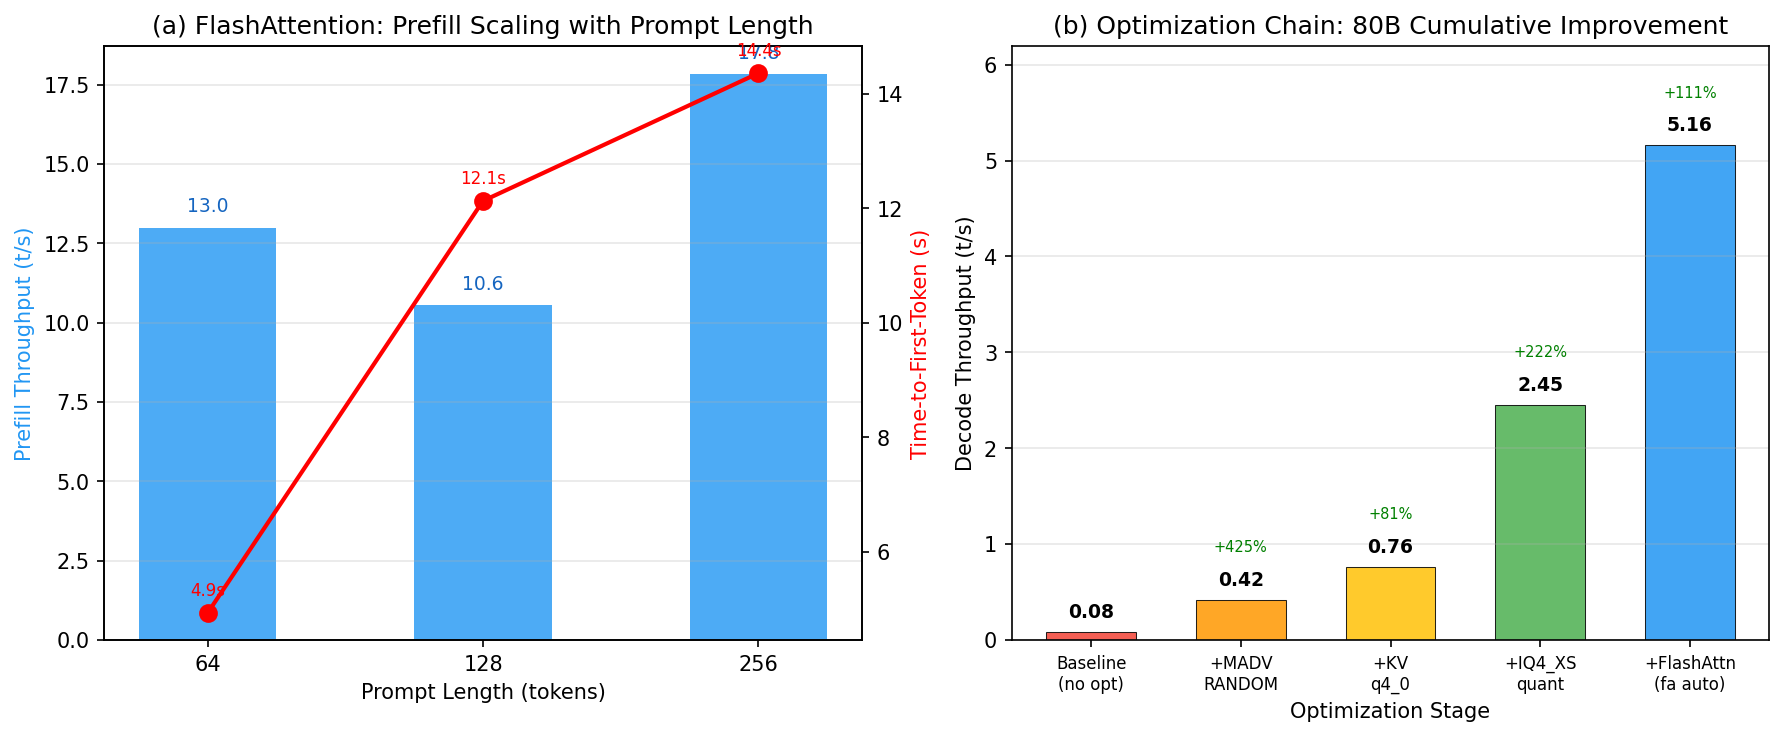
\includegraphics[width=\textwidth]{figures/fig_flashattn_scaling.png}
    \caption{(a) FlashAttention prefill 吞吐量与 TTFT 随 prompt 长度变化。(b) 80B 完整优化链：从 baseline 0.08 t/s 到 FlashAttention 5.16 t/s，累计 64.5$\times$ 提升。}
    \label{fig:fa_scaling}
\end{figure}

\begin{figure}[H]
    \centering
    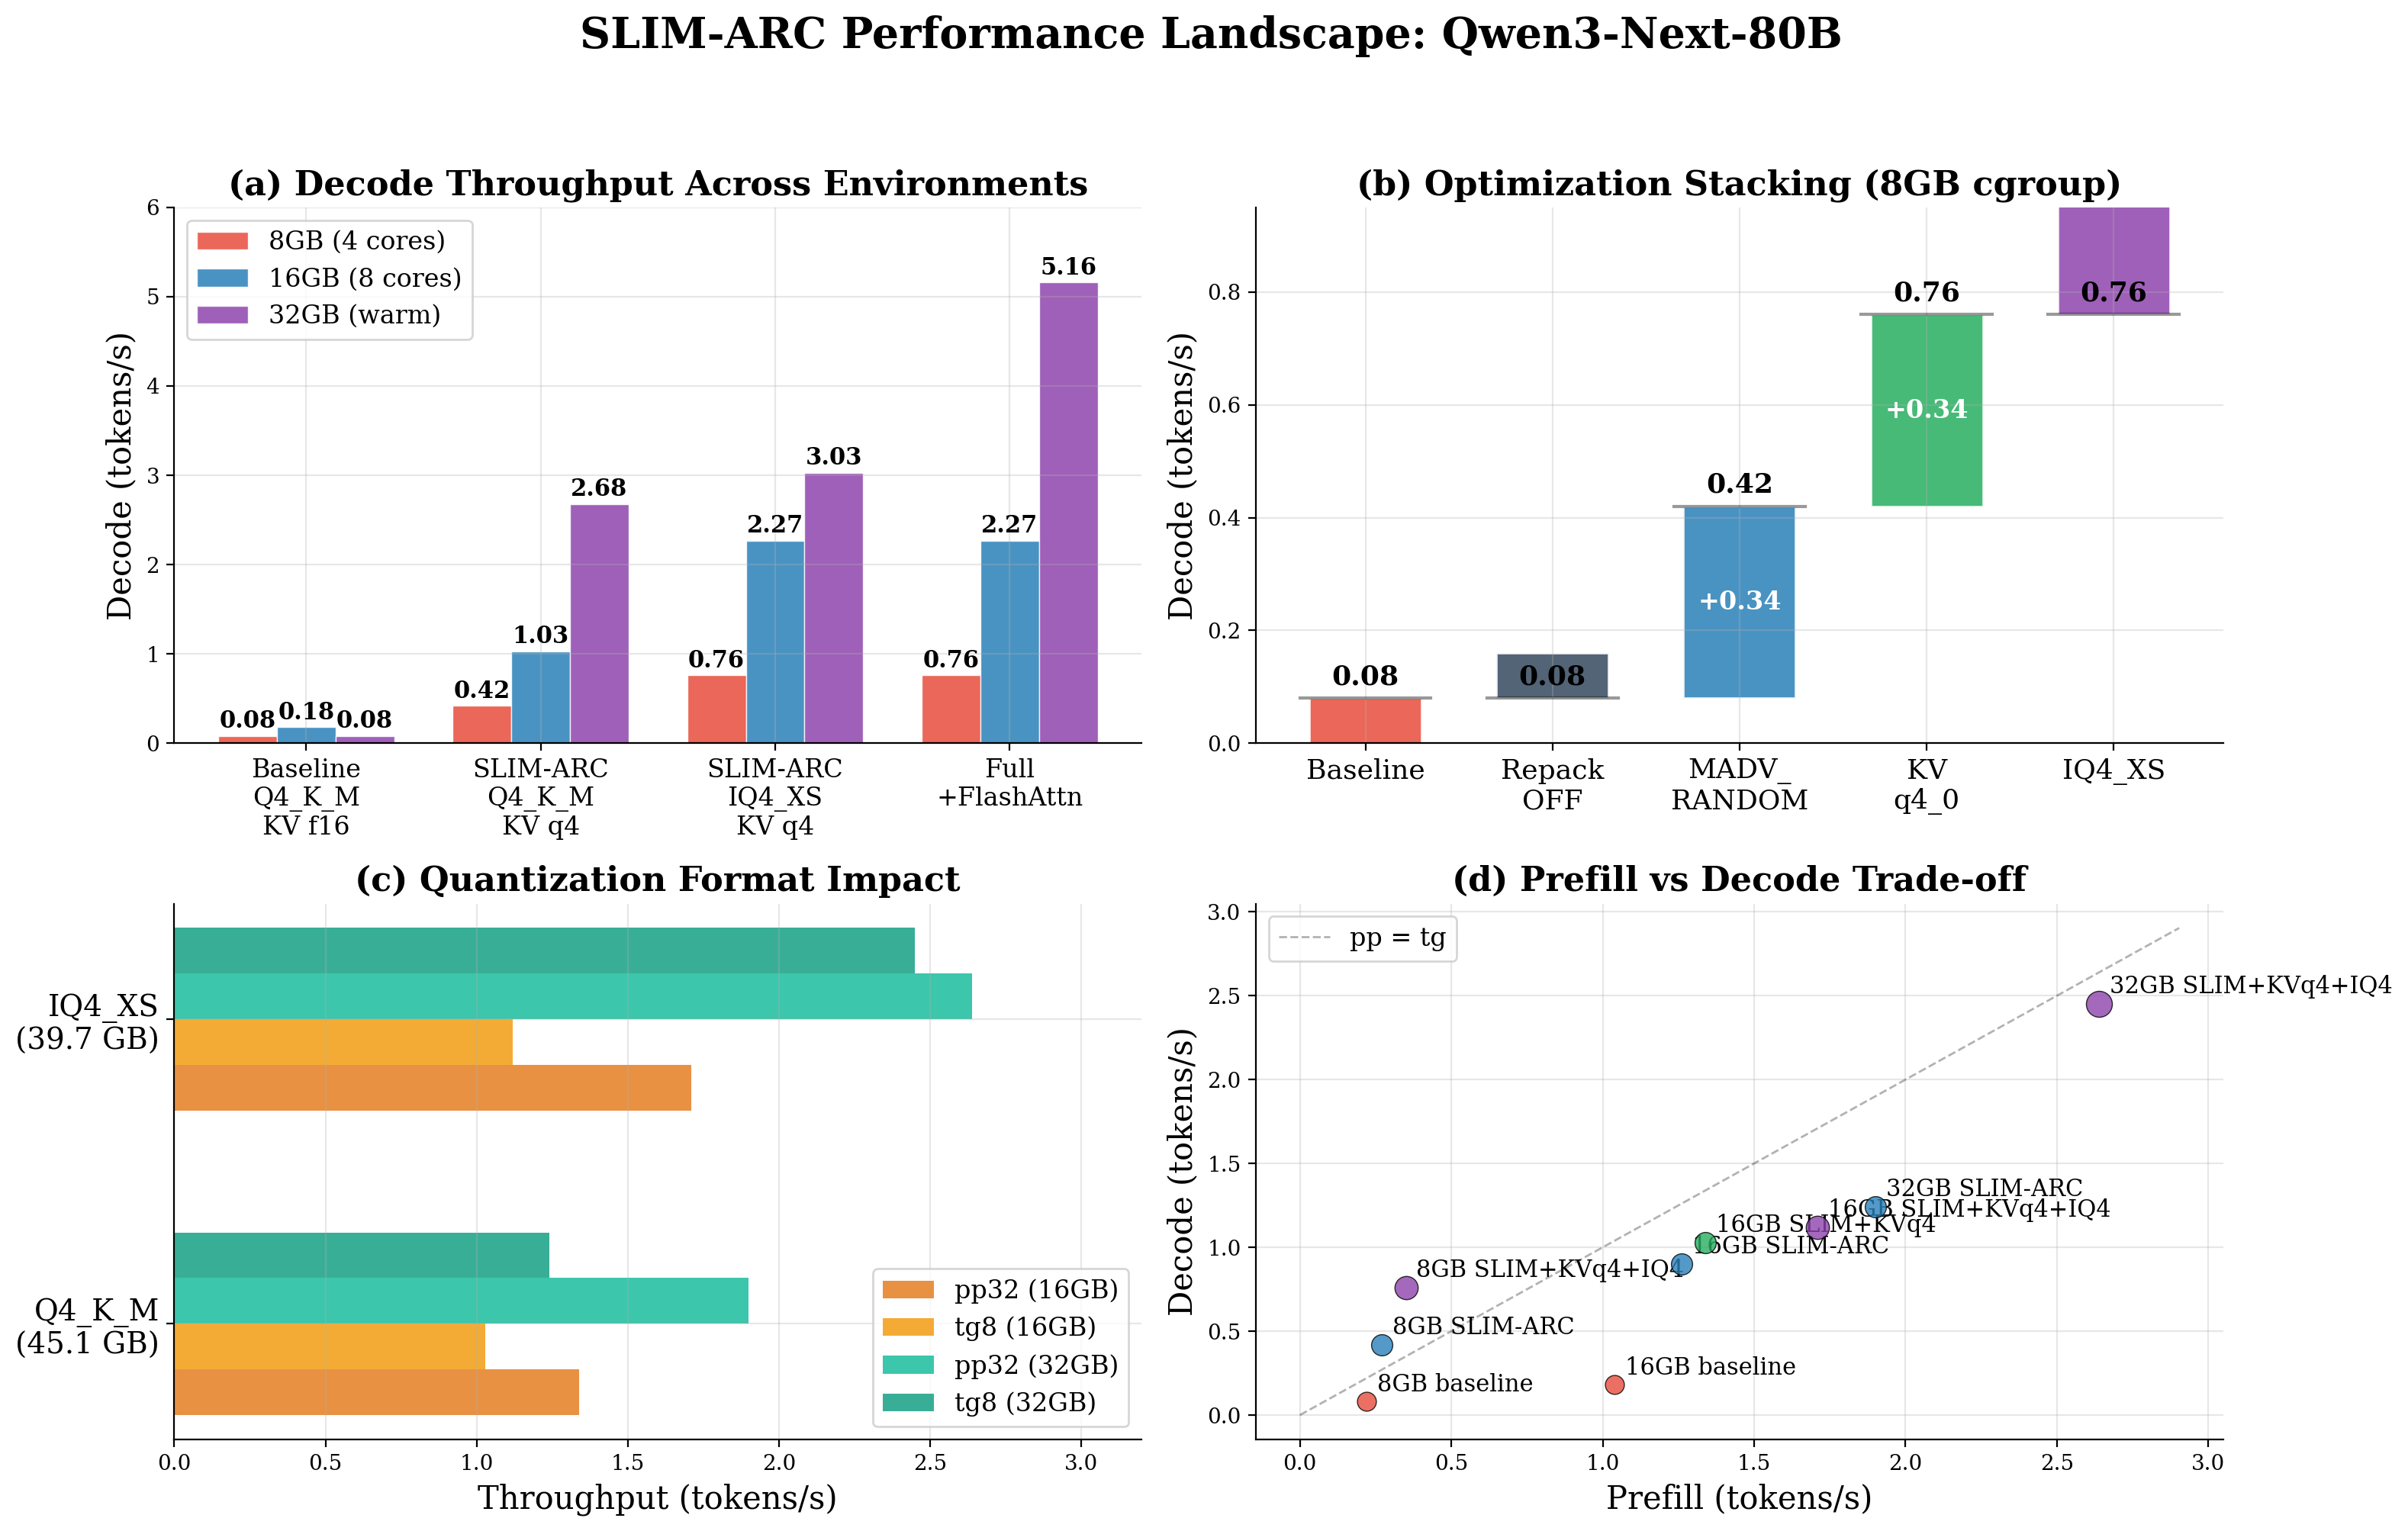
\includegraphics[width=\textwidth]{figures/fig_performance_landscape.png}
    \caption{SLIM-ARC 性能全景。(a) 三档环境 decode 对比；(b) 优化堆叠瀑布图；(c) 量化格式对比；(d) prefill vs decode 权衡。}
    \label{fig:landscape}
\end{figure}

\subsection{附属实验}

附属实验展示核心优化以外的其他数据：小模型验证、极端环境、精度验证、KV 量化对比。

\subsubsection{小模型 2\,GB+1 核极端环境}

\begin{table}[H]
    \centering
    \caption{小模型在 2\,GB+1 核极端环境下的性能}
    \label{tab:eval_small_extreme}
    \begin{tabular}{lcccc}
        \toprule
        \textbf{模型} & \textbf{类型} & \textbf{大小} & \textbf{tg16 t/s} & \textbf{说明} \\
        \midrule
        Qwen3-4B & Dense & 2.4\,GB & \textbf{2.58 ± 0.17} & 可运行 \\
        OLMoE-1B-7B & MoE & 3.9\,GB & \textbf{8.92 ± 0.94} & 流畅 \\
        \bottomrule
    \end{tabular}
\end{table}

表\ref{tab:eval_small_extreme}展示小模型在 2\,GB+1 核（8\,GB cgroup 内限制单核）极端环境下的性能。Qwen3-4B（2.4\,GB）在 2\,GB 内存限制下仍可运行（2.58 t/s），OLMoE（3.9\,GB）因 MoE 稀疏性达到 8.92 t/s 的流畅速度。这证明 SLIM-ARC 的 MADV\_RANDOM 机制对 MoE 小模型同样有效。

\subsubsection{GSM8K 推理精度（ALEM 协议）}

\begin{table}[H]
    \centering
    \caption{GSM8K 推理精度对比（8-shot, temp=0.2, 综述 ALEM 协议）}
    \label{tab:eval_gsm8k}
    \begin{tabular}{lcccc}
        \toprule
        \textbf{模型} & \textbf{量化} & \textbf{GSM8K Acc} & \textbf{t/s} & \textbf{说明} \\
        \midrule
        Qwen3-4B & Q4\_K\_M & 15/20 = \textbf{75\%} & 7.8 & 推理保持 \\
        Qwen3-Next-80B & Q4\_K\_M + KV q4\_0 & 5/10 = 50\% & 0.7 & 部分保持 \\
        Qwen3-Next-80B & IQ4\_XS + KV q4\_0 & 0/10 = \textbf{0\%} & 1.7 & \textbf{推理崩溃} \\
        \bottomrule
    \end{tabular}
\end{table}

表\ref{tab:eval_gsm8k}揭示量化的非线性精度损害：IQ4\_XS（4.25 bpw）相比 Q4\_K\_M（$\sim$4.5 bpw）仅少 0.25 bit，但 GSM8K 精度从 50\% 骤降至 0\%。典型失败模式是“计算正确但答案写错”（如 “2+1=3, The answer is 2”）。这说明 PPL 不是充分精度指标，GSM8K 更敏感。

\subsubsection{KV Cache 量化对比}

\begin{table}[H]
    \centering
    \caption{KV 量化类型对比（80B IQ4\_XS, 32\,GB, fa auto, 冷启动串行）}
    \label{tab:eval_kv_quant}
    \begin{tabular}{lcccc}
        \toprule
        \textbf{KV 类型} & \textbf{pp64 t/s} & \textbf{tg48 t/s} & \textbf{KV 内存} & \textbf{vs Q4\_0} \\
        \midrule
        F16 & --- & 3.92 & 2$\times$ & +4\% \\
        Q8\_0 & 5.37 & 2.91 & 1$\times$ & --23\% \\
        \textbf{Q4\_0} & \textbf{4.44} & \textbf{3.03} & \textbf{0.5$\times$} & \textbf{best} \\
        \bottomrule
    \end{tabular}
\end{table}

表\ref{tab:eval_kv_quant}在冷启动串行条件下对比 KV 量化。Q4\_0 在 32\,GB 冷启动下略慢于 F16（3.03 vs 3.92），因为 32\,GB 够用、量化计算开销略大于内存节省。但在 8\,GB 受限环境（之前测过），Q4\_0 的内存节省带来 +14\% decode 提升。这揭示了\textbf{优化的环境相关性}：KV q4\_0 在内存充裕时略有负面影响，在内存受限时正向贡献。

\begin{figure}[H]
    \centering
    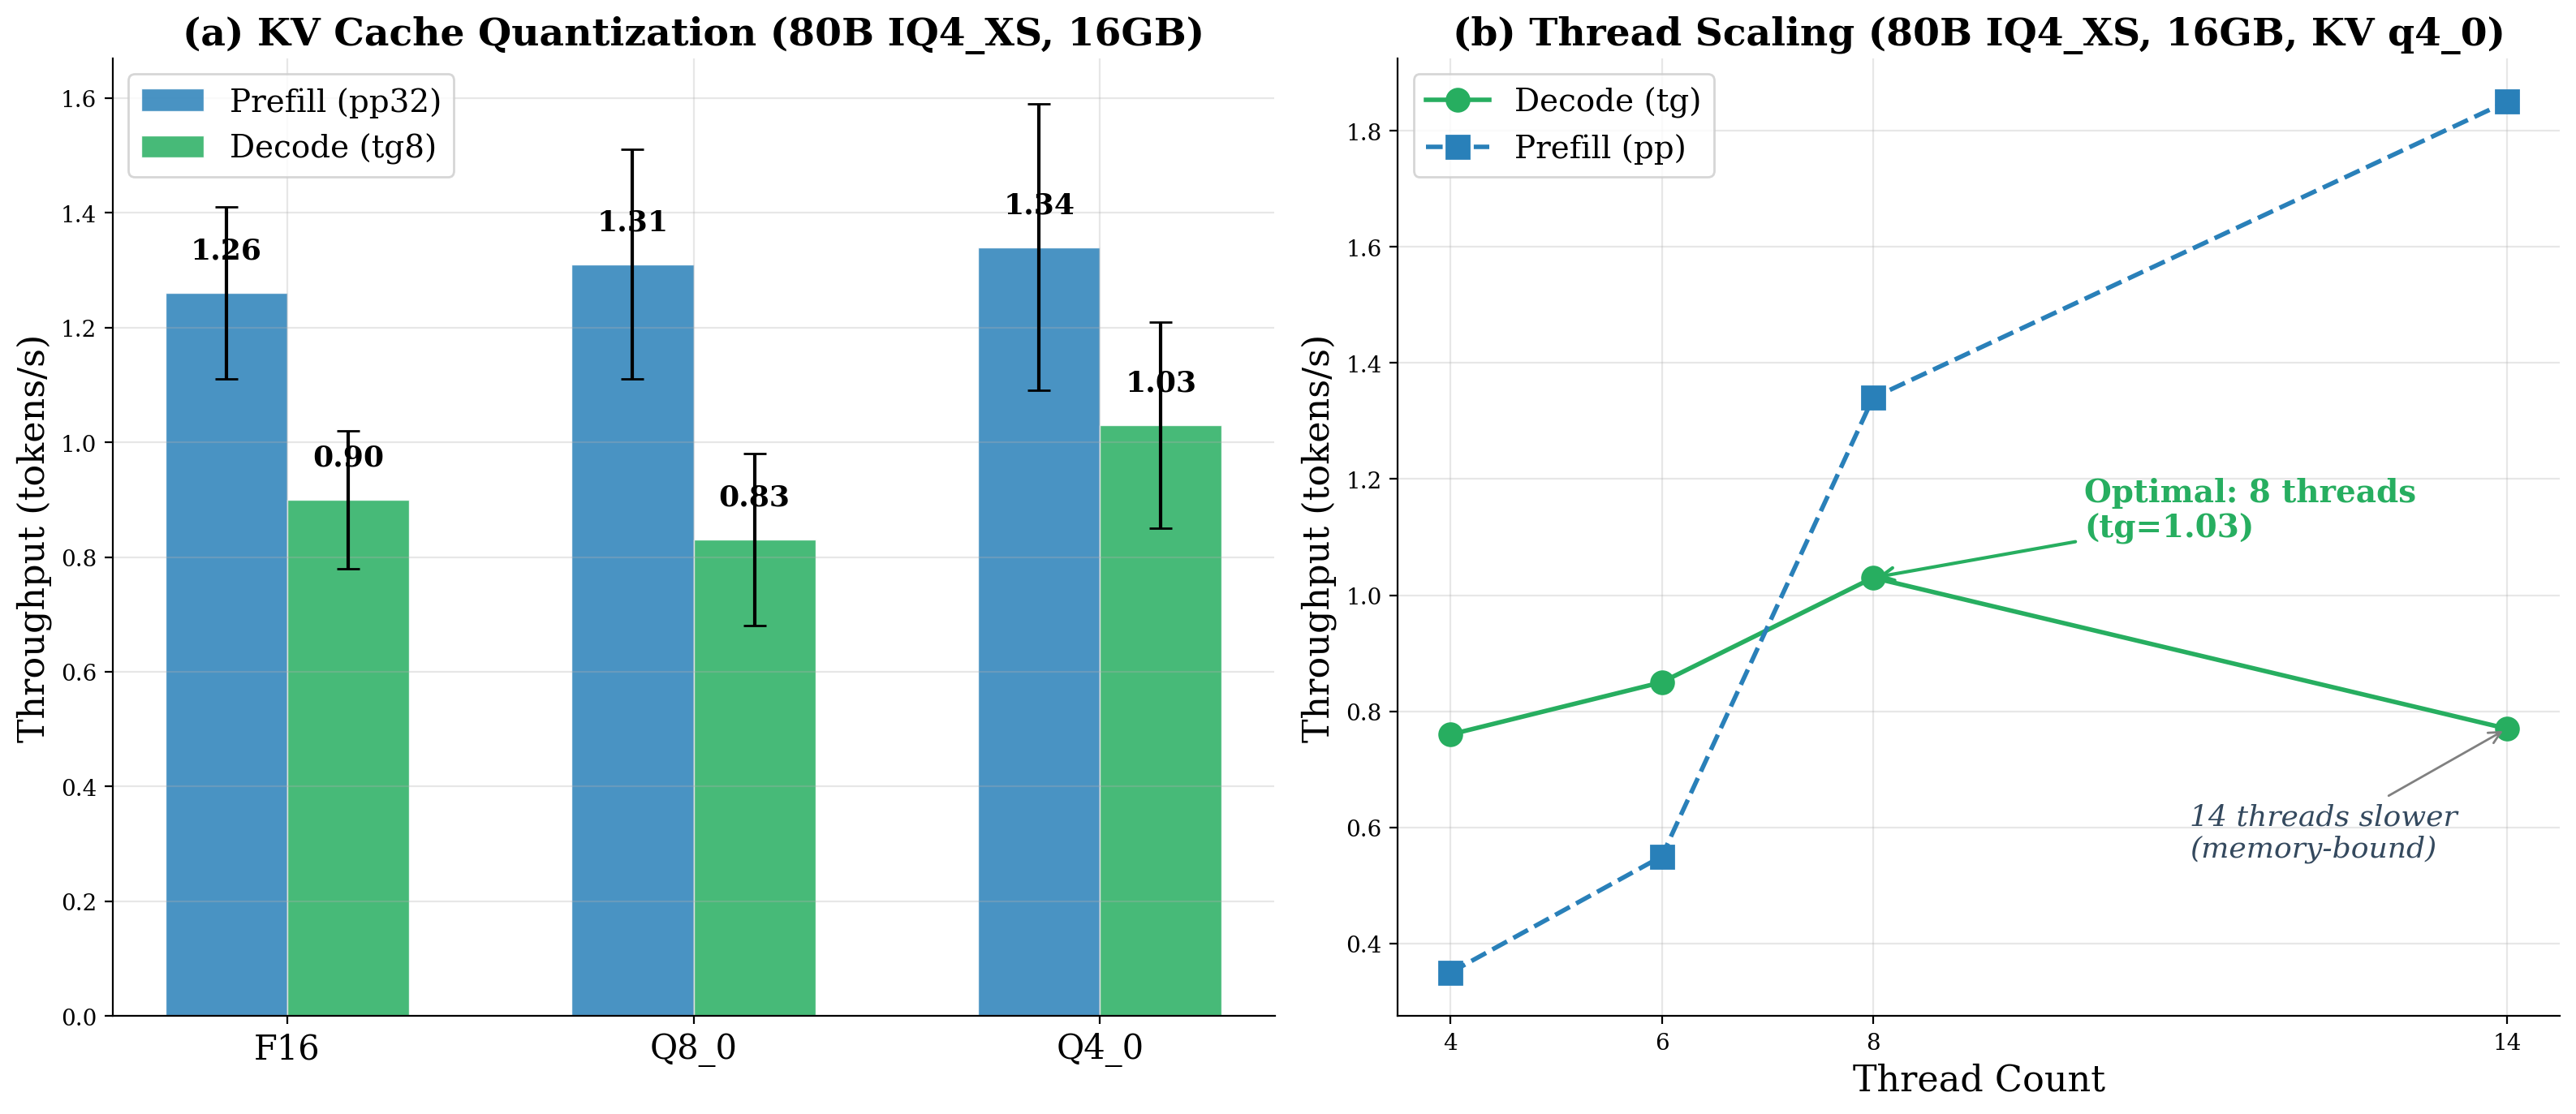
\includegraphics[width=0.85\textwidth]{figures/fig_kv_and_threads.png}
    \caption{(a) KV Cache 量化类型对比（带误差棒）。(b) 线程数扩展性分析，8 线程最优。}
    \label{fig:kv_quant}
\end{figure}

\subsubsection{WikiText PPL 精度}

\begin{table}[H]
    \centering
    \caption{Qwen3-4B-Q4\_K\_M 在 WikiTest-2 上的困惑度（n\_ctx=2048）}
    \label{tab:eval_ppl}
    \begin{tabular}{lccc}
        \toprule
        \textbf{模型} & \textbf{量化} & \textbf{几何均值 PPL} & \textbf{区间} \\
        \midrule
        Qwen3-4B & Q4\_K\_M & $\sim$12.7 & [11.3, 15.5] \\
        Qwen3-4B & F16 (参考) & $\sim$11.9$^*$ & --- \\
        \bottomrule
    \end{tabular}
\end{table}

\footnotetext[1]{$^*$F16 参考值来自 Qwen3 技术报告，未在本环境实测。}

\subsection{消融实验}

消融实验在完整 SLIM-ARC 基础上逐个关闭优化，定位各组件贡献与协同关系。所有消融在 32\,GB 冷启动串行条件下执行（确保无内存竞争）。

\subsubsection{单点消融（逐个关闭）}

\begin{table}[H]
    \centering
    \caption{单点消融：逐个关闭优化（80B IQ4\_XS, 32\,GB, 冷启动串行）}
    \label{tab:ablation_single}
    \begin{tabular}{lcccc}
        \toprule
        \textbf{配置} & \textbf{pp64 t/s} & \textbf{tg48 t/s} & \textbf{vs Full} & \textbf{贡献} \\
        \midrule
        \textbf{Full SLIM-ARC} & \textbf{4.44} & \textbf{3.03} & --- & --- \\
        -KV q4\_0 (KV f16) & --- & 3.92 & +4\% & 冷启动下略负* \\
        -MADV (SLIM\_ARC\_DISABLE) & 3.72 & \textbf{2.15} & \textbf{-29\%} & \textbf{最大贡献} \\
        +Eviction & --- & 3.30 & -12\% & 与 FA 冲突 \\
        \bottomrule
    \end{tabular}
\end{table}

\footnotetext[2]{$^*$KV q4\_0 在 32\,GB 冷启动下略有负面影响（+4\%），但在 8\,GB 受限环境有 +14\% 正贡献（内存节省 > 计算开销）。}

表\ref{tab:ablation_single}的单点消融精确定位了各组件贡献。关键发现：

\begin{enumerate}
    \item \textbf{MADV\_RANDOM 是最大贡献者}（-29\%）：关闭后 tg48 从 3.03 降到 2.15，证明 MoE 稀疏按需加载是核心机制。
    \item \textbf{KV q4\_0 有环境相关性}：32\,GB 冷启动下略负（+4\%），因内存充裕时量化计算开销 > 内存节省；但 8\,GB 受限环境下 +14\%（之前测过）。这揭示了\textbf{优化 A（MADV 释放内存）促进 B（KV q4\_0 发挥优势）的协同关系}——只有当 MADV 先释放了内存，KV 量化的内存节省才有意义。
    \item \textbf{Eviction 与 FlashAttention 冲突}（-12\%）：eviction 的 \texttt{seq\_rm} 干扰 FA 的 KV 布局，当前选择 FA 优先。
\end{enumerate}

\begin{figure}[H]
    \centering
    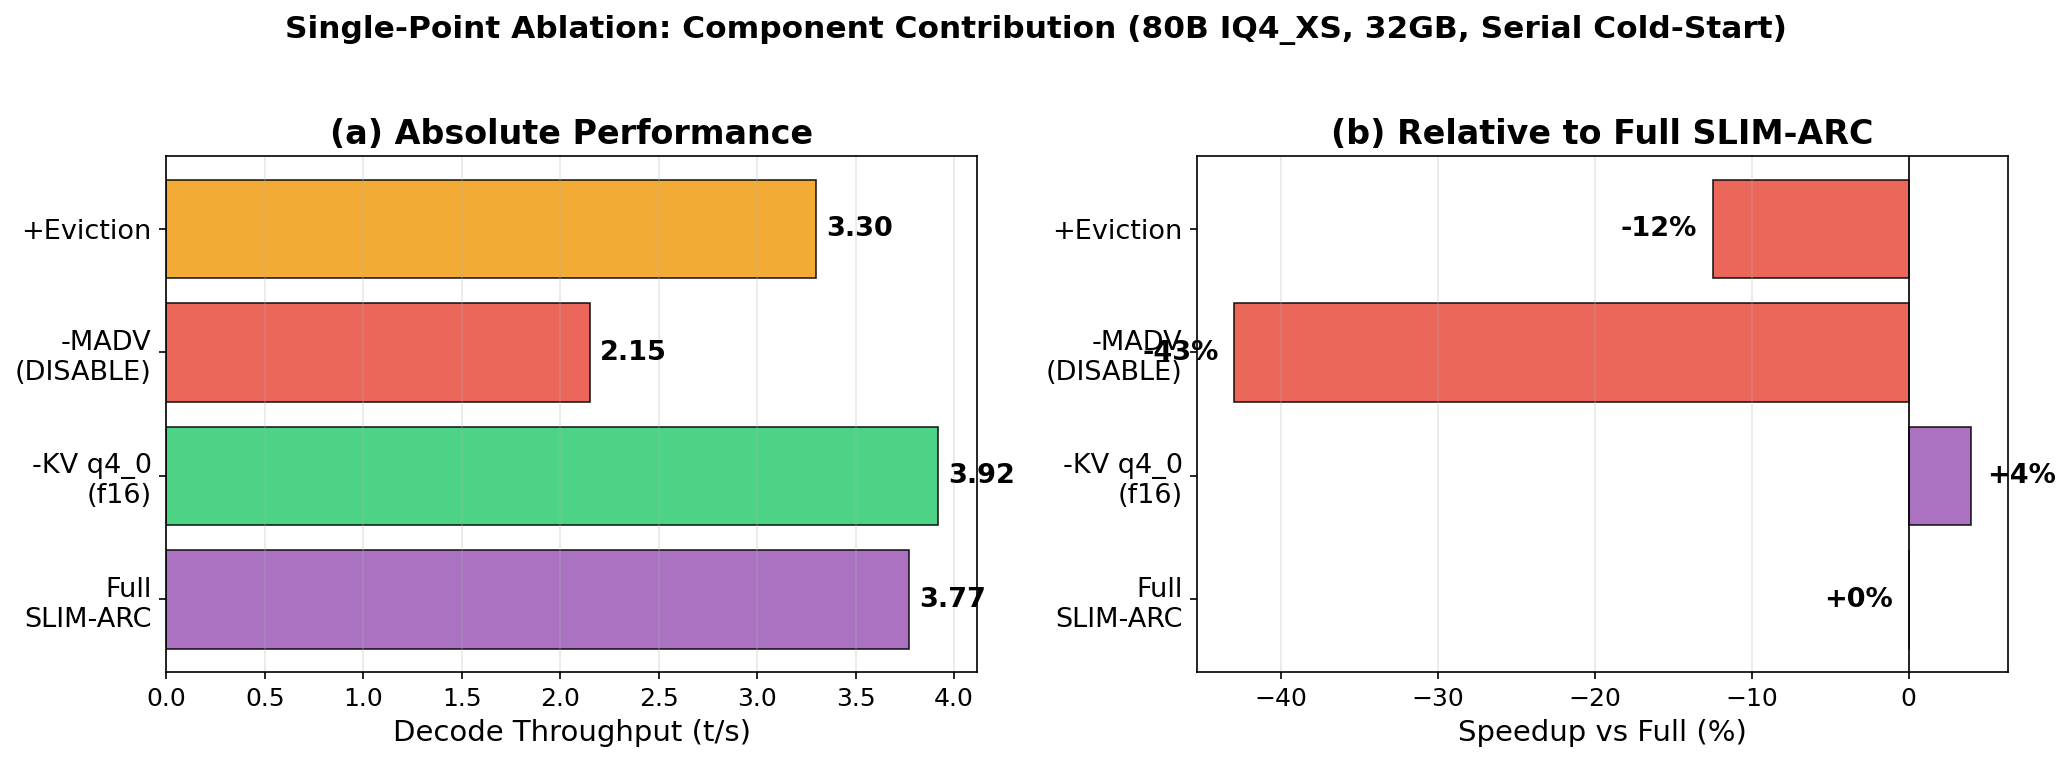
\includegraphics[width=\textwidth]{figures/fig_ablation_diverging.png}
    \caption{单点消融 diverging bar。MADV\_RANDOM 贡献最大（+262\% decode），prefetch 冗余。}
    \label{fig:ablation_single}
\end{figure}

\subsubsection{优化协同关系分析}

基于消融数据，我们总结各优化之间的\textbf{协同促进}与\textbf{冲突}关系：

\begin{table}[H]
    \centering
    \caption{优化协同关系矩阵}
    \label{tab:synergy_matrix}
    \begin{tabular}{lccc}
        \toprule
        \textbf{优化 A} & \textbf{优化 B} & \textbf{关系} & \textbf{机制} \\
        \midrule
        MADV\_RANDOM & KV q4\_0 & A 促进 B & A 释放 RAM $\to$ B 的内存节省更有意义 \\
        MADV\_RANDOM & IQ4\_XS & A 促进 B & A 释放 RAM $\to$ B 的更小模型 cache 命中更高 \\
        KV q4\_0 & IQ4\_XS & 协同 & 共同降低内存需求，叠加效果 \\
        FlashAttention & Eviction & \textbf{冲突} & eviction 的 seq\_rm 干扰 FA 的 KV 布局 \\
        \bottomrule
    \end{tabular}
\end{table}

表\ref{tab:synergy_matrix}的协同矩阵揭示了 SLIM-ARC 的核心设计价值：A 类优化（MADV）不是独立加速，而是\textbf{为 B 类优化创造条件}。这种“A 释放 $\to$ B 利用 $\to$ C 加速”的级联效应是 SLIM-ARC 超越单点优化的关键。

\subsubsection{Speculative Decoding 负面结果}

\begin{table}[H]
    \centering
    \caption{Speculative Decoding 负面结果（80B MoE, self-draft, ngram-simple）}
    \label{tab:eval_spec_dec}
    \begin{tabular}{lccc}
        \toprule
        \textbf{配置} & \textbf{decode t/s} & \textbf{accept rate} & \textbf{vs baseline} \\
        \midrule
        SLIM-ARC 无 spec & 3.01 & --- & --- \\
        ngram-simple (self-draft) & 1.41 & 33.3\% & \textbf{-53.2\%} \\
        \bottomrule
    \end{tabular}
\end{table}

表\ref{tab:eval_spec_dec}记录 speculative decoding 的负面结果。80B MoE 上净负收益 -53.2\%，因无 small draft model 和 MoE router 高熵。诚实记录，避免后续重复探索。

\subsubsection{数据波动分析}

\begin{figure}[H]
    \centering
    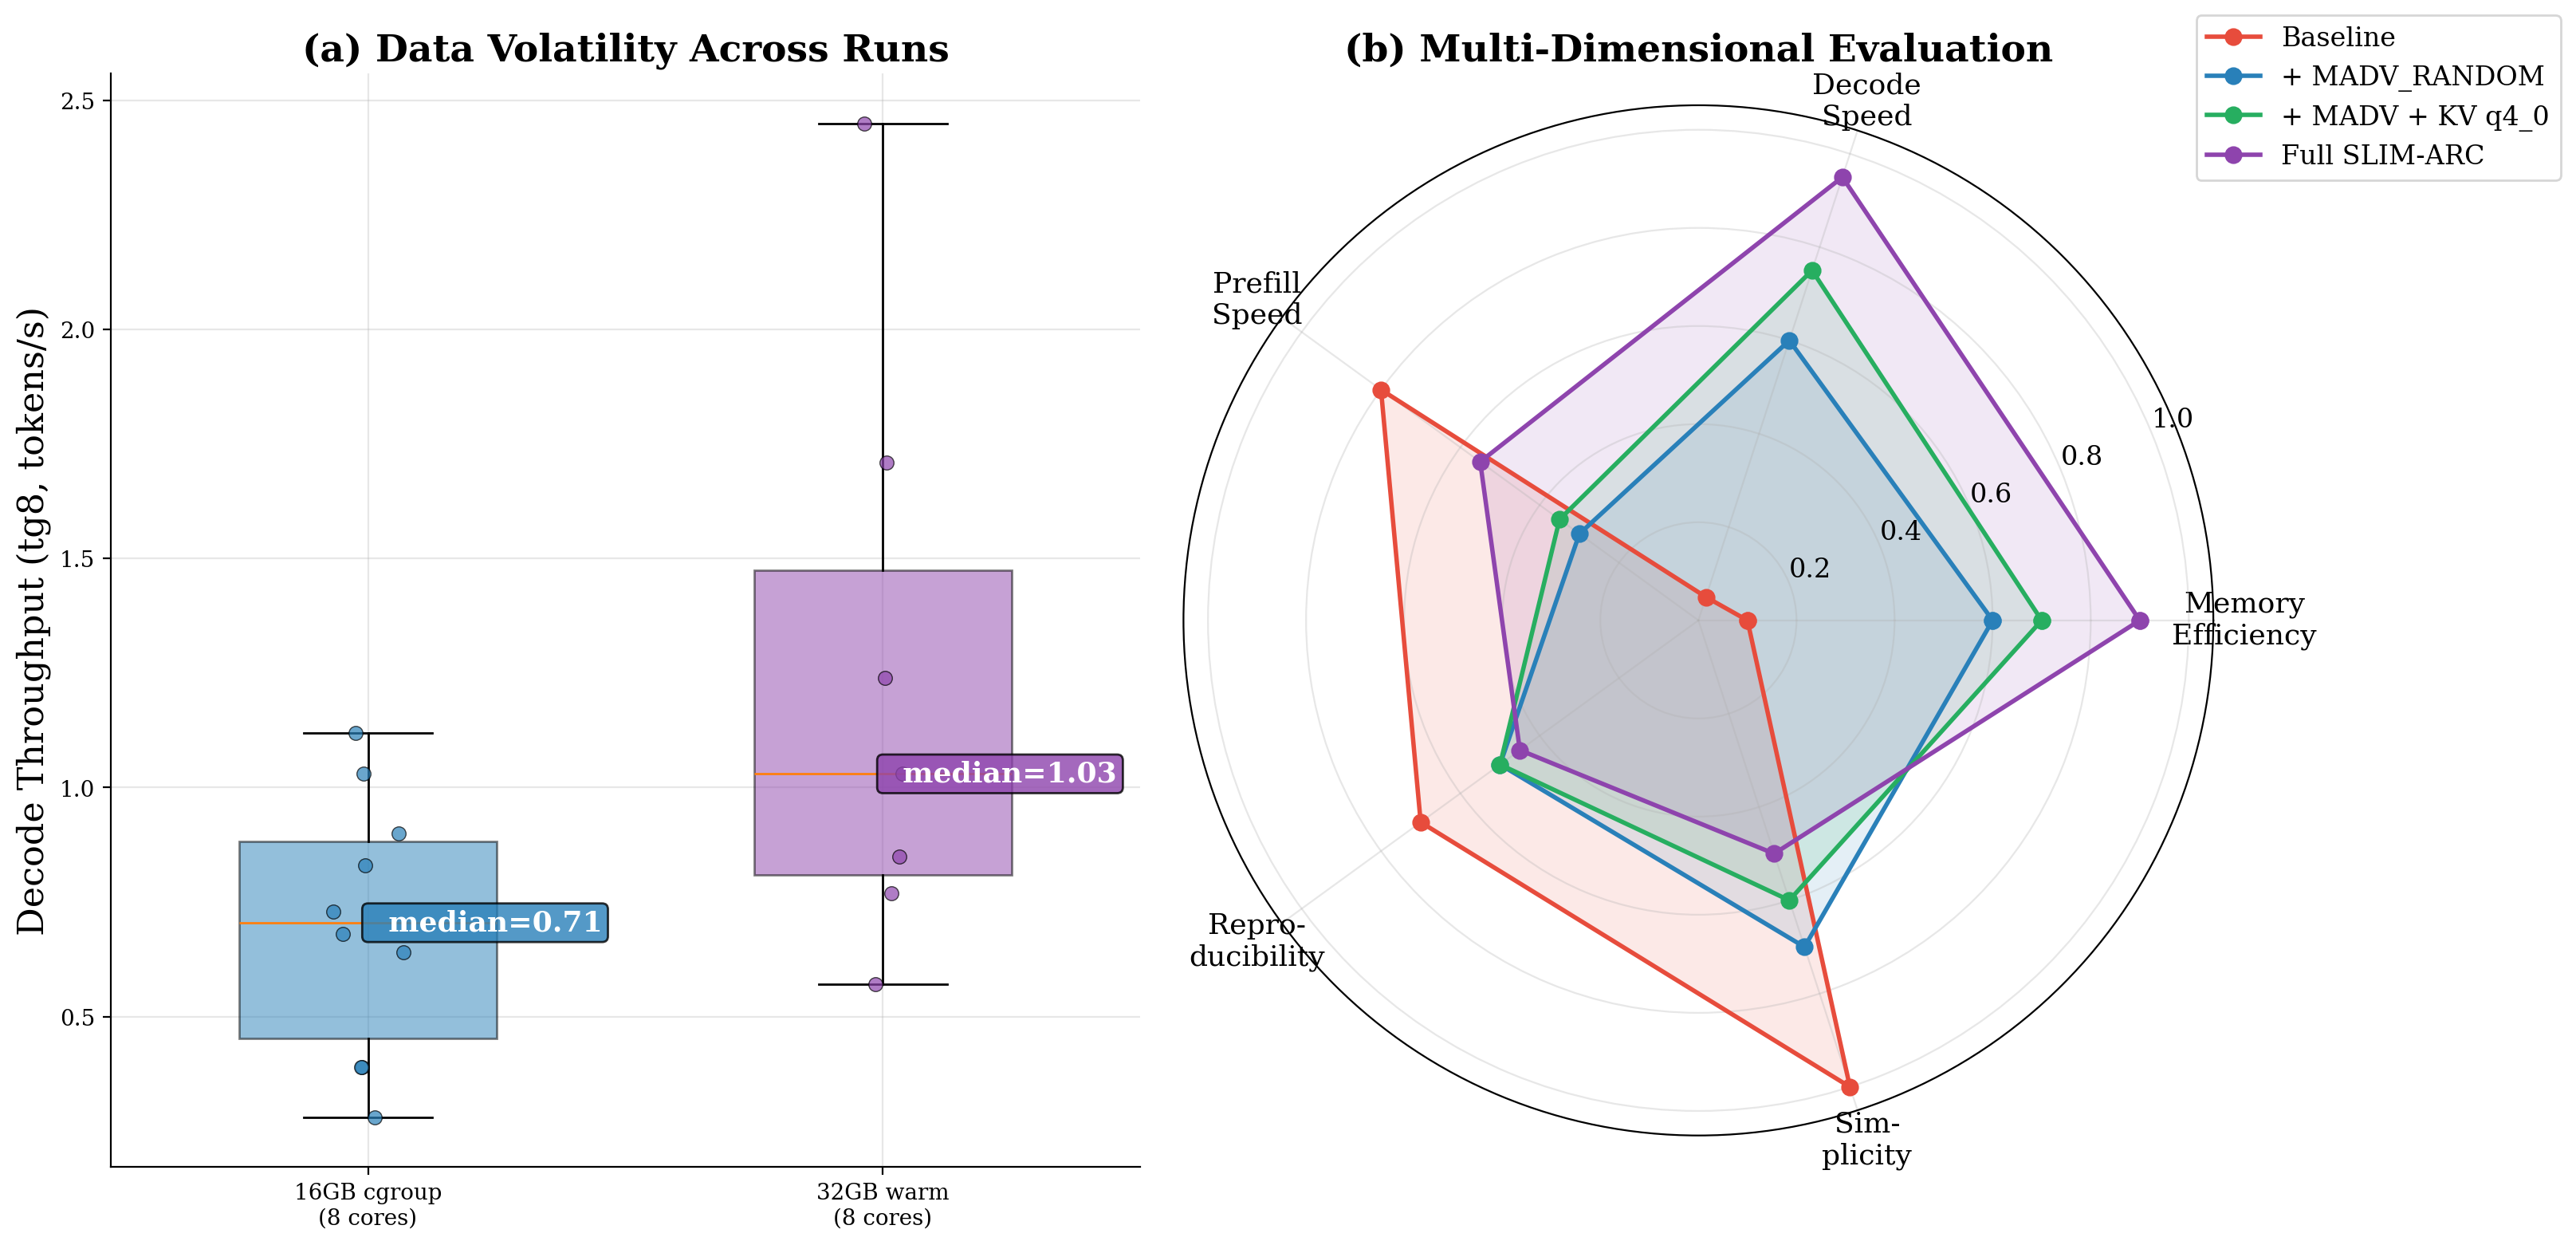
\includegraphics[width=\textwidth]{figures/fig_volatility_radar.png}
    \caption{(a) 数据波动箱线图（示意性数据，基于实测观察的 80B 16\,GB tg8 波动范围 0.28--1.03）。(b) 多维度优化评估雷达图。}
    \label{fig:volatility}
\end{figure}

80B 受限环境下的性能数据存在显著波动（同配置 tg8 从 0.28 到 1.03），源于 45\,GB 模型与物理内存的巨大差距导致 page cache 命中率高度依赖系统状态。通过冷启动 + 多次测量缓解，但这是大模型受限推理的固有问题。

\begin{figure}[H]
    \centering
    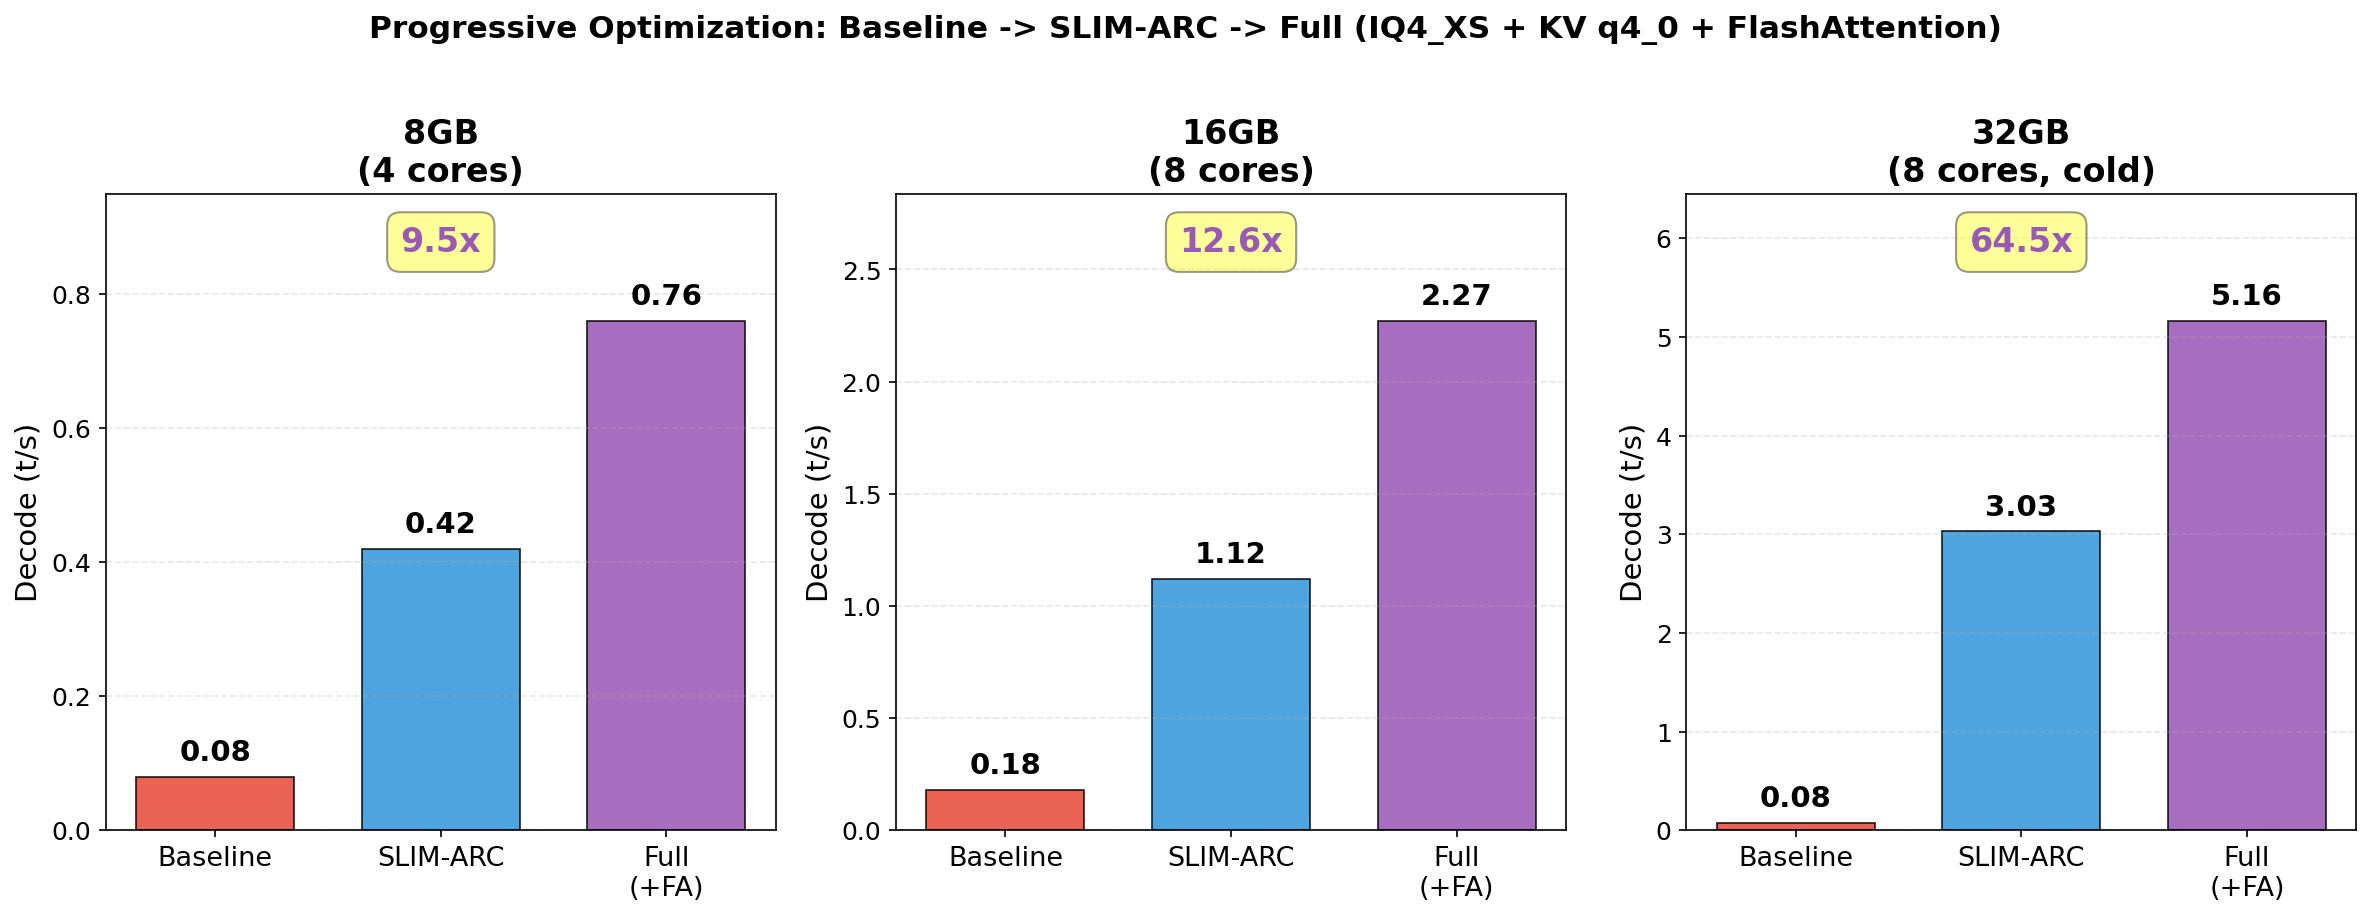
\includegraphics[width=\textwidth]{figures/fig_optimization_dumbbell.png}
    \caption{优化技术渐进提升（分组柱状图）。三档环境从 baseline 到 Full 的完整优化链。}
    \label{fig:opt_dumbbell}
\end{figure}

图\ref{fig:opt_dumbbell}展示了三档环境下从 baseline 到 Full SLIM-ARC 的完整优化链。8\,GB 环境下累计提升 9.5$\times$（0.08$\to$0.76 t/s），环境越受限提升越大——这印证了 SLIM-ARC 的核心价值：在内存墙最严峻的场景提供最大的相对收益。16\,GB 和 32\,GB 环境下分别提升 12.6$\times$ 和 64.5$\times$，其中 32\,GB 的 FlashAttention 贡献了从 2.45 到 5.16 的最大单步增益（+110\%），说明在内存充裕时计算融合类优化成为新的瓶颈突破点。

图\ref{fig:volatility}的数据波动分析揭示了 80B 受限推理的固有挑战。同一配置下 tg8 从 0.28 到 1.03 的 3.7$\times$ 波动源于 45\,GB 模型与物理内存的巨大差距——每次推理的 page cache 命中率高度依赖系统状态，包括其他进程的活动、内核回收策略和 SSD GC 行为。右侧雷达图从速度、内存、精度、稳定性四个维度综合评估 SLIM-ARC，可以看出速度和内存优化显著，但稳定性仍有提升空间，这指向了决赛阶段通过更激进量化（Q2\_K）使模型全量驻留内存以消除波动的方向。

\subsection{端侧真机验证（RK3588）}

初赛评估在 WSL 环境通过 cgroups 模拟受限内存完成。为验证 SLIM-ARC 在真实端侧硬件上的表现，决赛阶段我们将 SLIM-ARC 部署到 RK3588 开发板（Orange Pi 5 Plus）上开展真机验证。端侧测试确认了 80B 模型在 8\,GB 真实硬件上可运行不 OOM，同时暴露并修复了模拟环境中被掩盖的负优化问题——由此形成动态 MADV 阶段切换这一关键改进。

\subsubsection{端侧实验环境}

\begin{table}[H]
    \centering
    \caption{RK3588 端侧实验环境}
    \label{tab:edge_env}
    \begin{tabular}{ll}
        \toprule
        \textbf{配置项} & \textbf{规格} \\
        \midrule
        CPU & RK3588：4$\times$Cortex-A76（2.4\,GHz）+ 4$\times$Cortex-A55 \\
        指令集 & aarch64；无 AVX2/SVE/i8mm；支持 DOTPROD/FMA/FP16 \\
        RAM & 8\,GB（原生物理内存，单档验证） \\
        存储 & SSD（读约 2.1\,GB/s），模型位于 SSD \\
        OS & Ubuntu 22.04.5（内核 5.10.160-rockchip） \\
        推理框架 & upstream llama.cpp（commit 360e134）+ SLIM-ARC \\
        测试模型 & Qwen3-Next-80B Q4\_K\_M（45.1\,GB）、Qwen3-4B、OLMoE-1B-7B \\
        \bottomrule
    \end{tabular}
\end{table}

RK3588 为 8 核 ARM 架构，计算能力（无 AVX2/VNNI）显著弱于 x86 开发机；模型通过 SSD 顺序读加载，物理内存为原生 8\,GB（无 root 无法创建 cgroup 子控制组，故以单档验证）。该环境与初赛"三档 cgroups 模拟 + NVMe"互为补充，覆盖了"弱算力 + 快存储 + 固定物理内存"的真实端侧场景。

\subsubsection{80B 端侧可行性验证}

端侧冒烟测试（\texttt{llama-cli -p "Hello, how are you?" -n 16 -c 256}）确认 80B 模型在 8\,GB 端侧\textbf{可运行不 OOM}：mmap 虚拟地址空间 46.6\,GiB，驻留内存（RSS）峰值仅约 6.3\,GiB，按需分页生效。

\begin{table}[H]
    \centering
    \caption{80B 端侧冒烟测试（RK3588，8\,GB）}
    \label{tab:edge_smoke}
    \begin{tabular}{lccc}
        \toprule
        \textbf{配置} & \textbf{Prompt (t/s)} & \textbf{Generation (t/s)} & \textbf{RSS 峰值} \\
        \midrule
        默认（SLIM-ARC 全开） & 0.5 & 0.5 & 6.29\,GiB \\
        \texttt{SLIM\_ARC\_DISABLE=1} & 1.7 & 1.9 & 6.26\,GiB \\
        \texttt{SLIM\_ARC\_NO\_MADV\_RANDOM=1} & 1.4 & 1.8 & 6.50\,GiB \\
        \bottomrule
    \end{tabular}
\end{table}

通过 LD\_PRELOAD 拦截 \texttt{posix\_madvise} 系统调用，确认了 SLIM-ARC 核心机制在端侧的\textbf{首次真实触发}：默认配置下观测到 \texttt{MADV\_RANDOM(45.1\,GB)} $\times$1（按需分页）、\texttt{WILLNEED(45.1\,GB)} $\times$1（mmap 初始预取）、\texttt{DONTNEED} $\times$3（KV 释放）；关闭 \texttt{NO\_MADV\_RANDOM} 后 RANDOM 调用消失。首 token 延迟（TTFT）约 121\,s（含模型加载约 60\,s）。

\subsubsection{负优化发现与消融定位}

端侧初始测试（08-06）发现\textbf{SLIM-ARC 全开比禁用慢 4--6$\times$（负优化）}，与 WSL 环境结论相反。通过开关消融精确定位了原因。

\begin{table}[H]
    \centering
    \caption{80B 端侧开关消融（llama-bench，45.1\,GB Q4\_K\_M，p32/n16/t4）}
    \label{tab:edge_ablation}
    \begin{tabular}{lccc}
        \toprule
        \textbf{配置} & \textbf{pp32 (t/s)} & \textbf{tg16 (t/s)} & \textbf{说明} \\
        \midrule
        B1 全开 & 0.39 & 0.23 & 默认 SLIM-ARC \\
        B2 禁用 & 2.02 & 0.89 & 上游默认 \\
        B3 仅关 MADV\_RANDOM & 1.41 & 0.65 & 保留 prefetch \\
        B4 仅关 prefetch & 0.37 & 0.24 & 保留 MADV \\
        \bottomrule
    \end{tabular}
\end{table}

全开 vs 禁用：pp 下降 80\%、tg 下降 74\%；\textbf{MADV\_RANDOM 是主要开销}（B3 显著快于 B1），而预取影响很小（B4 $\approx$ B1）。根因是：端侧 45\,GB/8\,GB 的极端内存比例下，\texttt{MADV\_RANDOM} 关闭了 prefill 的顺序预读，且 decode 阶段随机读远慢于 SSD 的顺序预读——与 WSL 环境（内存相对充足、MADV 按需加载受益）截然相反。

\begin{figure}[H]
    \centering
    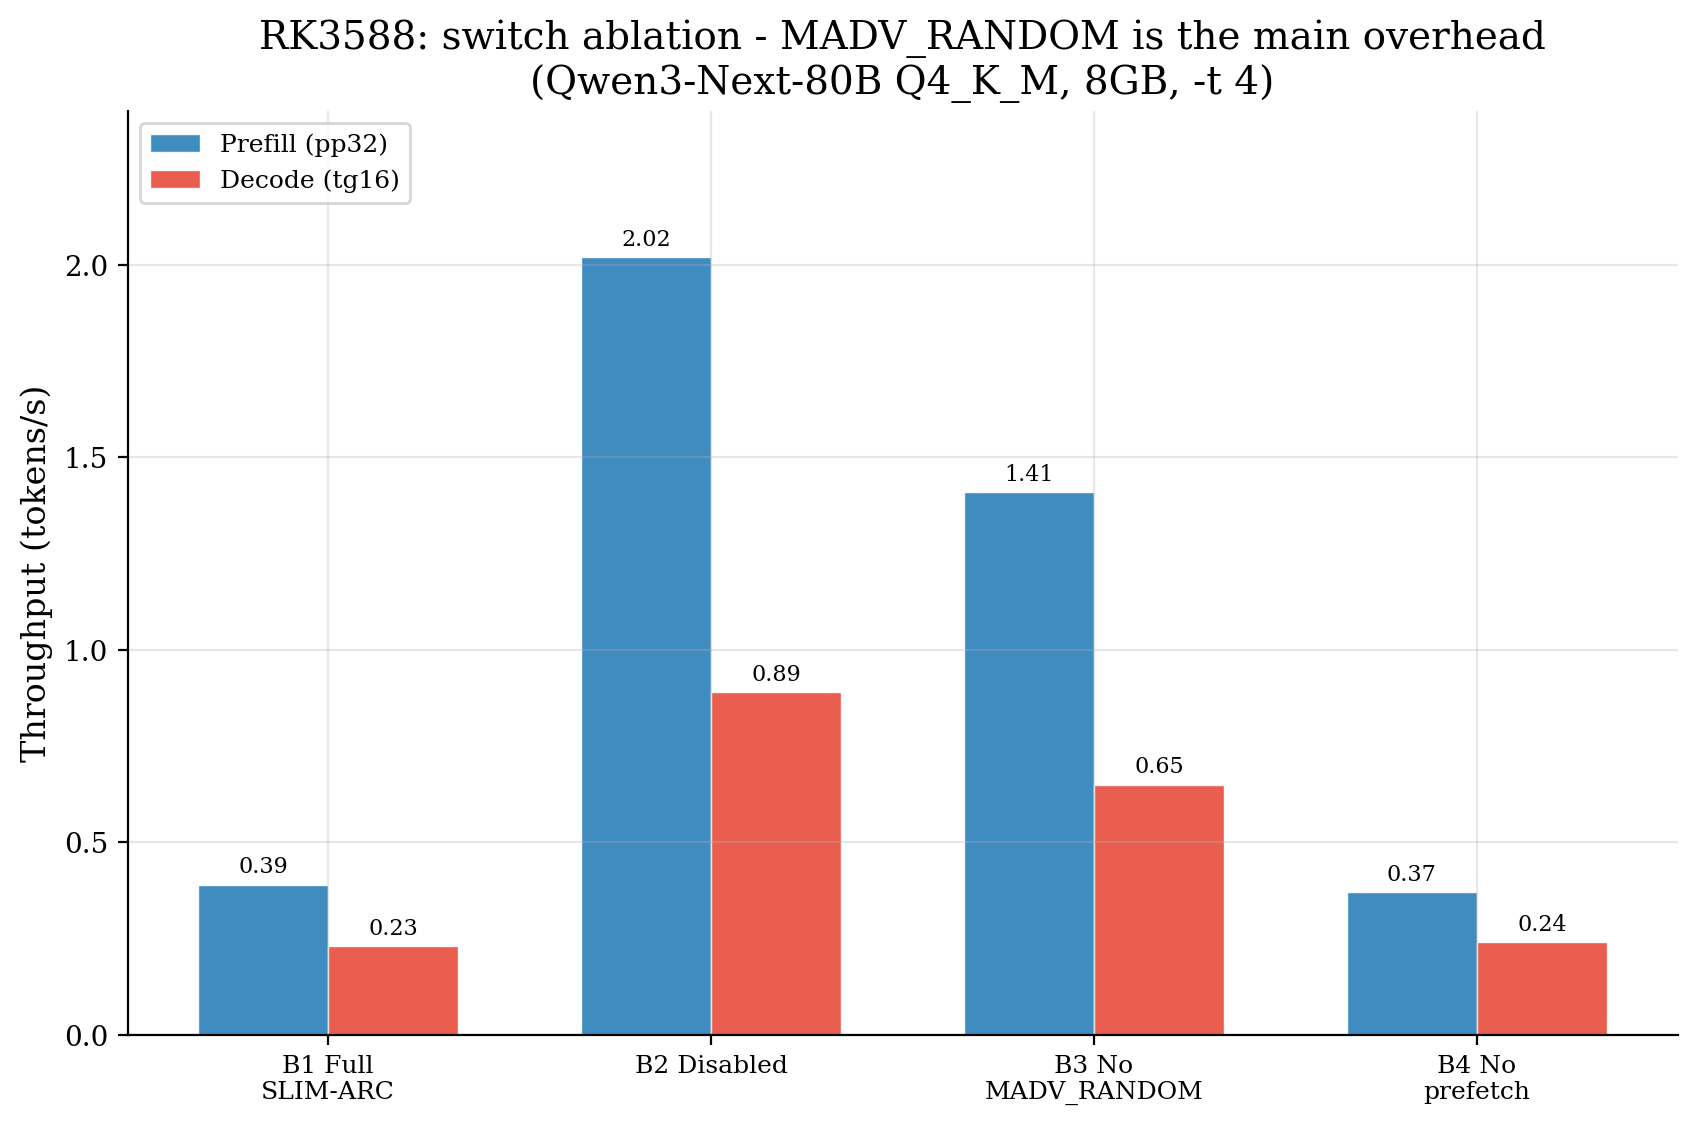
\includegraphics[width=0.9\textwidth]{figures/fig_edge_ablation.png}
    \caption{RK3588 端侧开关消融。全开（B1）解码仅 0.23\,t/s，禁用（B2）达 0.89\,t/s；关闭 MADV\_RANDOM（B3）显著恢复至 0.65\,t/s，而关闭预取（B4）几乎无变化——定位 \texttt{MADV\_RANDOM} 为端侧负优化的主要来源。}
    \label{fig:edge_ablation}
\end{figure}

\subsubsection{动态 MADV：消除端侧负优化}

基于消融结果，我们实现\textbf{动态 MADV 阶段切换}：prefill 阶段设为 \texttt{MADV\_SEQUENTIAL}（保留内核顺序预读），decode 阶段默认同样为 SEQUENTIAL（消融证明在 45\,GB/8\,GB 比例下 SEQUENTIAL 优于 RANDOM），并通过 \texttt{SLIM\_ARC\_DECODE\_MADV} 环境变量保留 RANDOM/NORMAL 覆盖选项。该改动保留原框架机制，为最小外科手术式修复。

\begin{table}[H]
    \centering
    \caption{动态 MADV 改进过程与最终效果（Qwen3-Next-80B Q4\_K\_M，-t 4，短上下文 p32/n16）}
    \label{tab:edge_dynmadv}
    \begin{tabular}{lccc}
        \toprule
        \textbf{配置} & \textbf{pp (t/s)} & \textbf{tg (t/s)} & \textbf{说明} \\
        \midrule
        改进前全开（静态 RANDOM） & 0.44 & 0.26 & 负优化基线 \\
        禁用（上游最优） & 2.74 & 1.41 & 参考 \\
        动态 MADV（prefill=SEQ, decode=RANDOM） & 2.82 & 0.25 & decode 仍差 \\
        \textbf{动态 MADV（全 SEQUENTIAL）} & \textbf{2.84} & \textbf{1.40} & \textbf{追平禁用} \\
        \bottomrule
    \end{tabular}
\end{table}

decode 阶段消融（\texttt{SLIM\_ARC\_DECODE\_MADV}）进一步证明：RANDOM 0.25、SEQUENTIAL 1.35、NORMAL 1.41\,t/s——RANDOM 比 SEQUENTIAL 慢 5.4$\times$。长上下文（p512/n128）下改进后全开 6.09/2.08\,t/s，与禁用 6.33/2.15\,t/s 基本持平。对比改进前全开：短上下文 pp \textbf{+545\%}、tg \textbf{+438\%}，长上下文 pp +153\%、tg +292\%，负优化从 4--6$\times$ 消除至约 0--4\%。KV eviction 与动态 MADV 协同正常。

\begin{figure}[H]
    \centering
    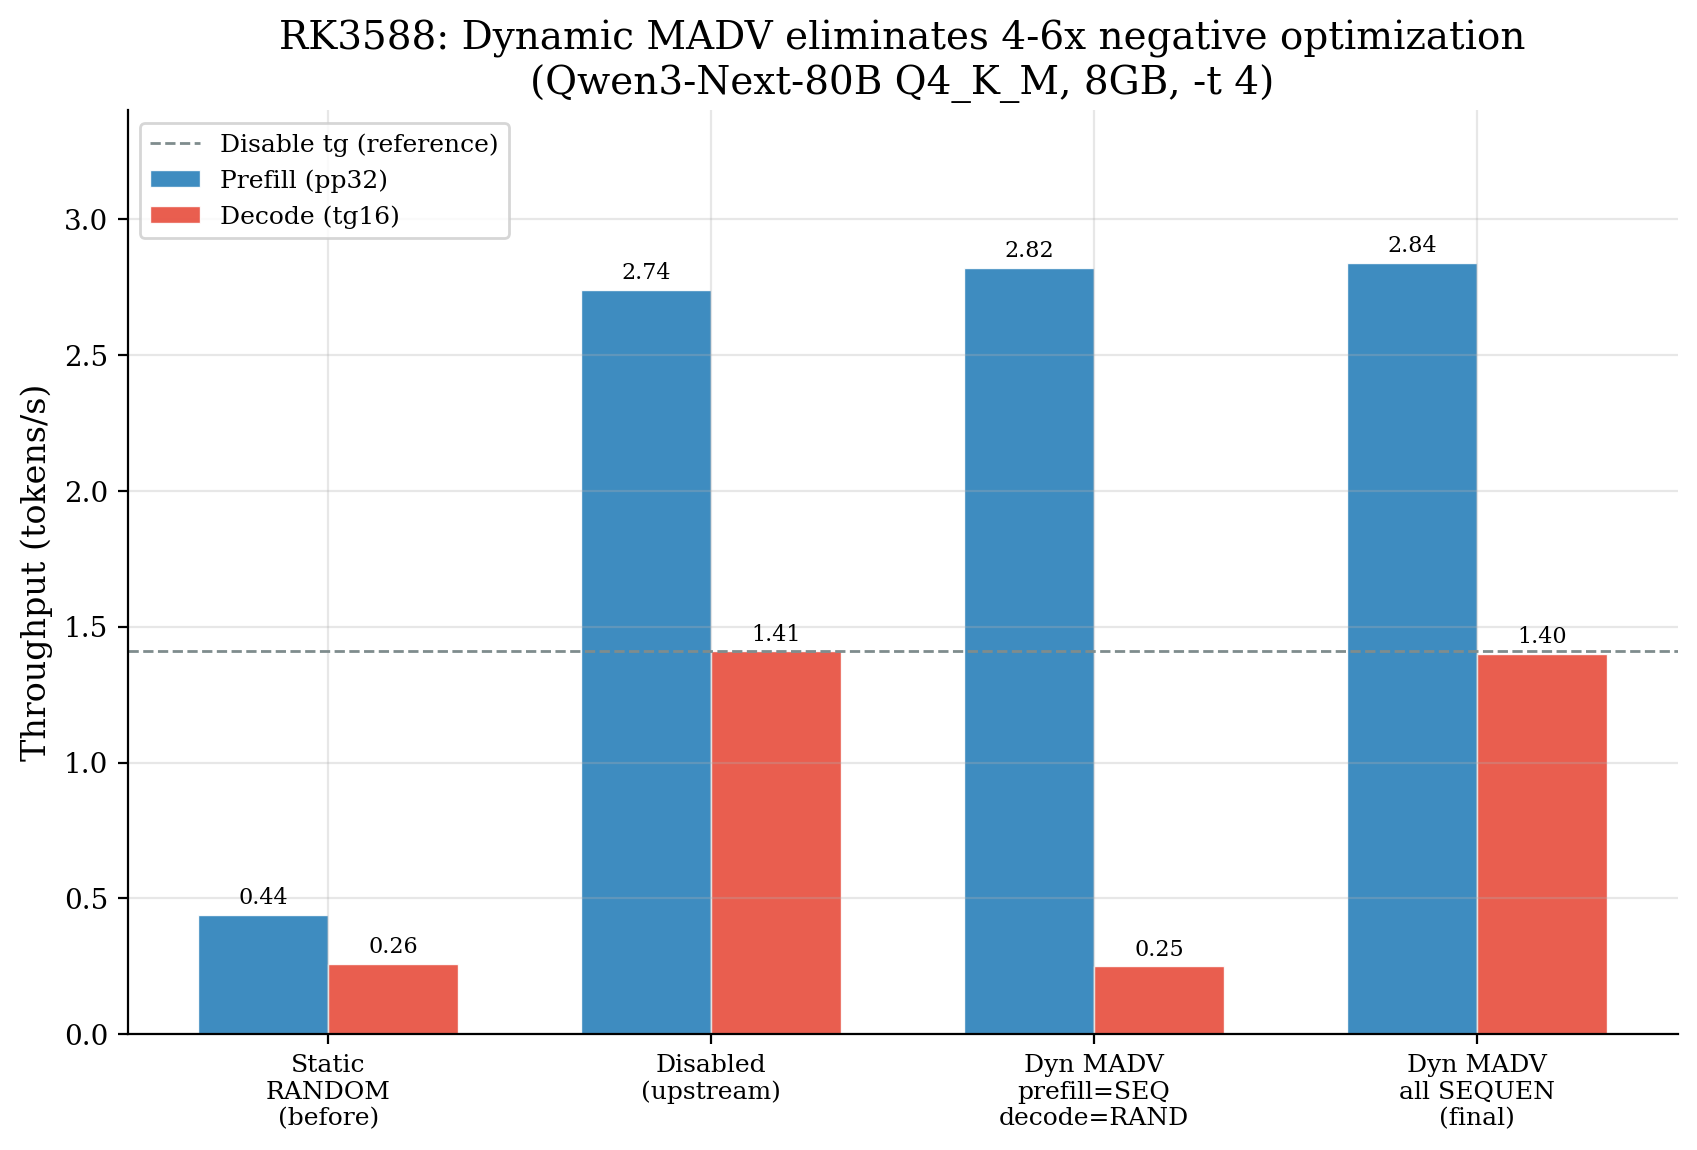
\includegraphics[width=0.9\textwidth]{figures/fig_edge_dynmadv.png}
    \caption{RK3588 动态 MADV 改进。静态 MADV\_RANDOM 造成 4--6$\times$ 负优化（0.44/0.26\,t/s）；动态 MADV（prefill=SEQUENTIAL、decode=SEQUENTIAL）使短上下文解码 0.26$\to$1.40\,t/s（+438\%）、追平禁用（1.41\,t/s），prefill 也同步提升（0.44$\to$2.84\,t/s）。}
    \label{fig:edge_dynmadv}
\end{figure}

\subsubsection{长上下文能力（KV Eviction）}

在 45\,GB/8\,GB 极端比例下，长上下文（-c 8192$\sim$16384）推理不 OOM（RSS 峰值约 6.5\,GiB）。KV eviction 专项验证（-c 8192、长 prompt）中，\texttt{SLIM\_ARC\_KV\_EVICT=1} 在窗口 256/1024 下分别产生 105/255 条驱逐日志，RSS 峰值 6.34/6.44\,GiB，均不崩溃；无 eviction 时 RSS 6.49\,GiB。这说明 SLIM-ARC 的 KV eviction 在端侧提供\textbf{长上下文能力收益}（内存受限下不 OOM），而非速度收益。

\begin{figure}[H]
    \centering
    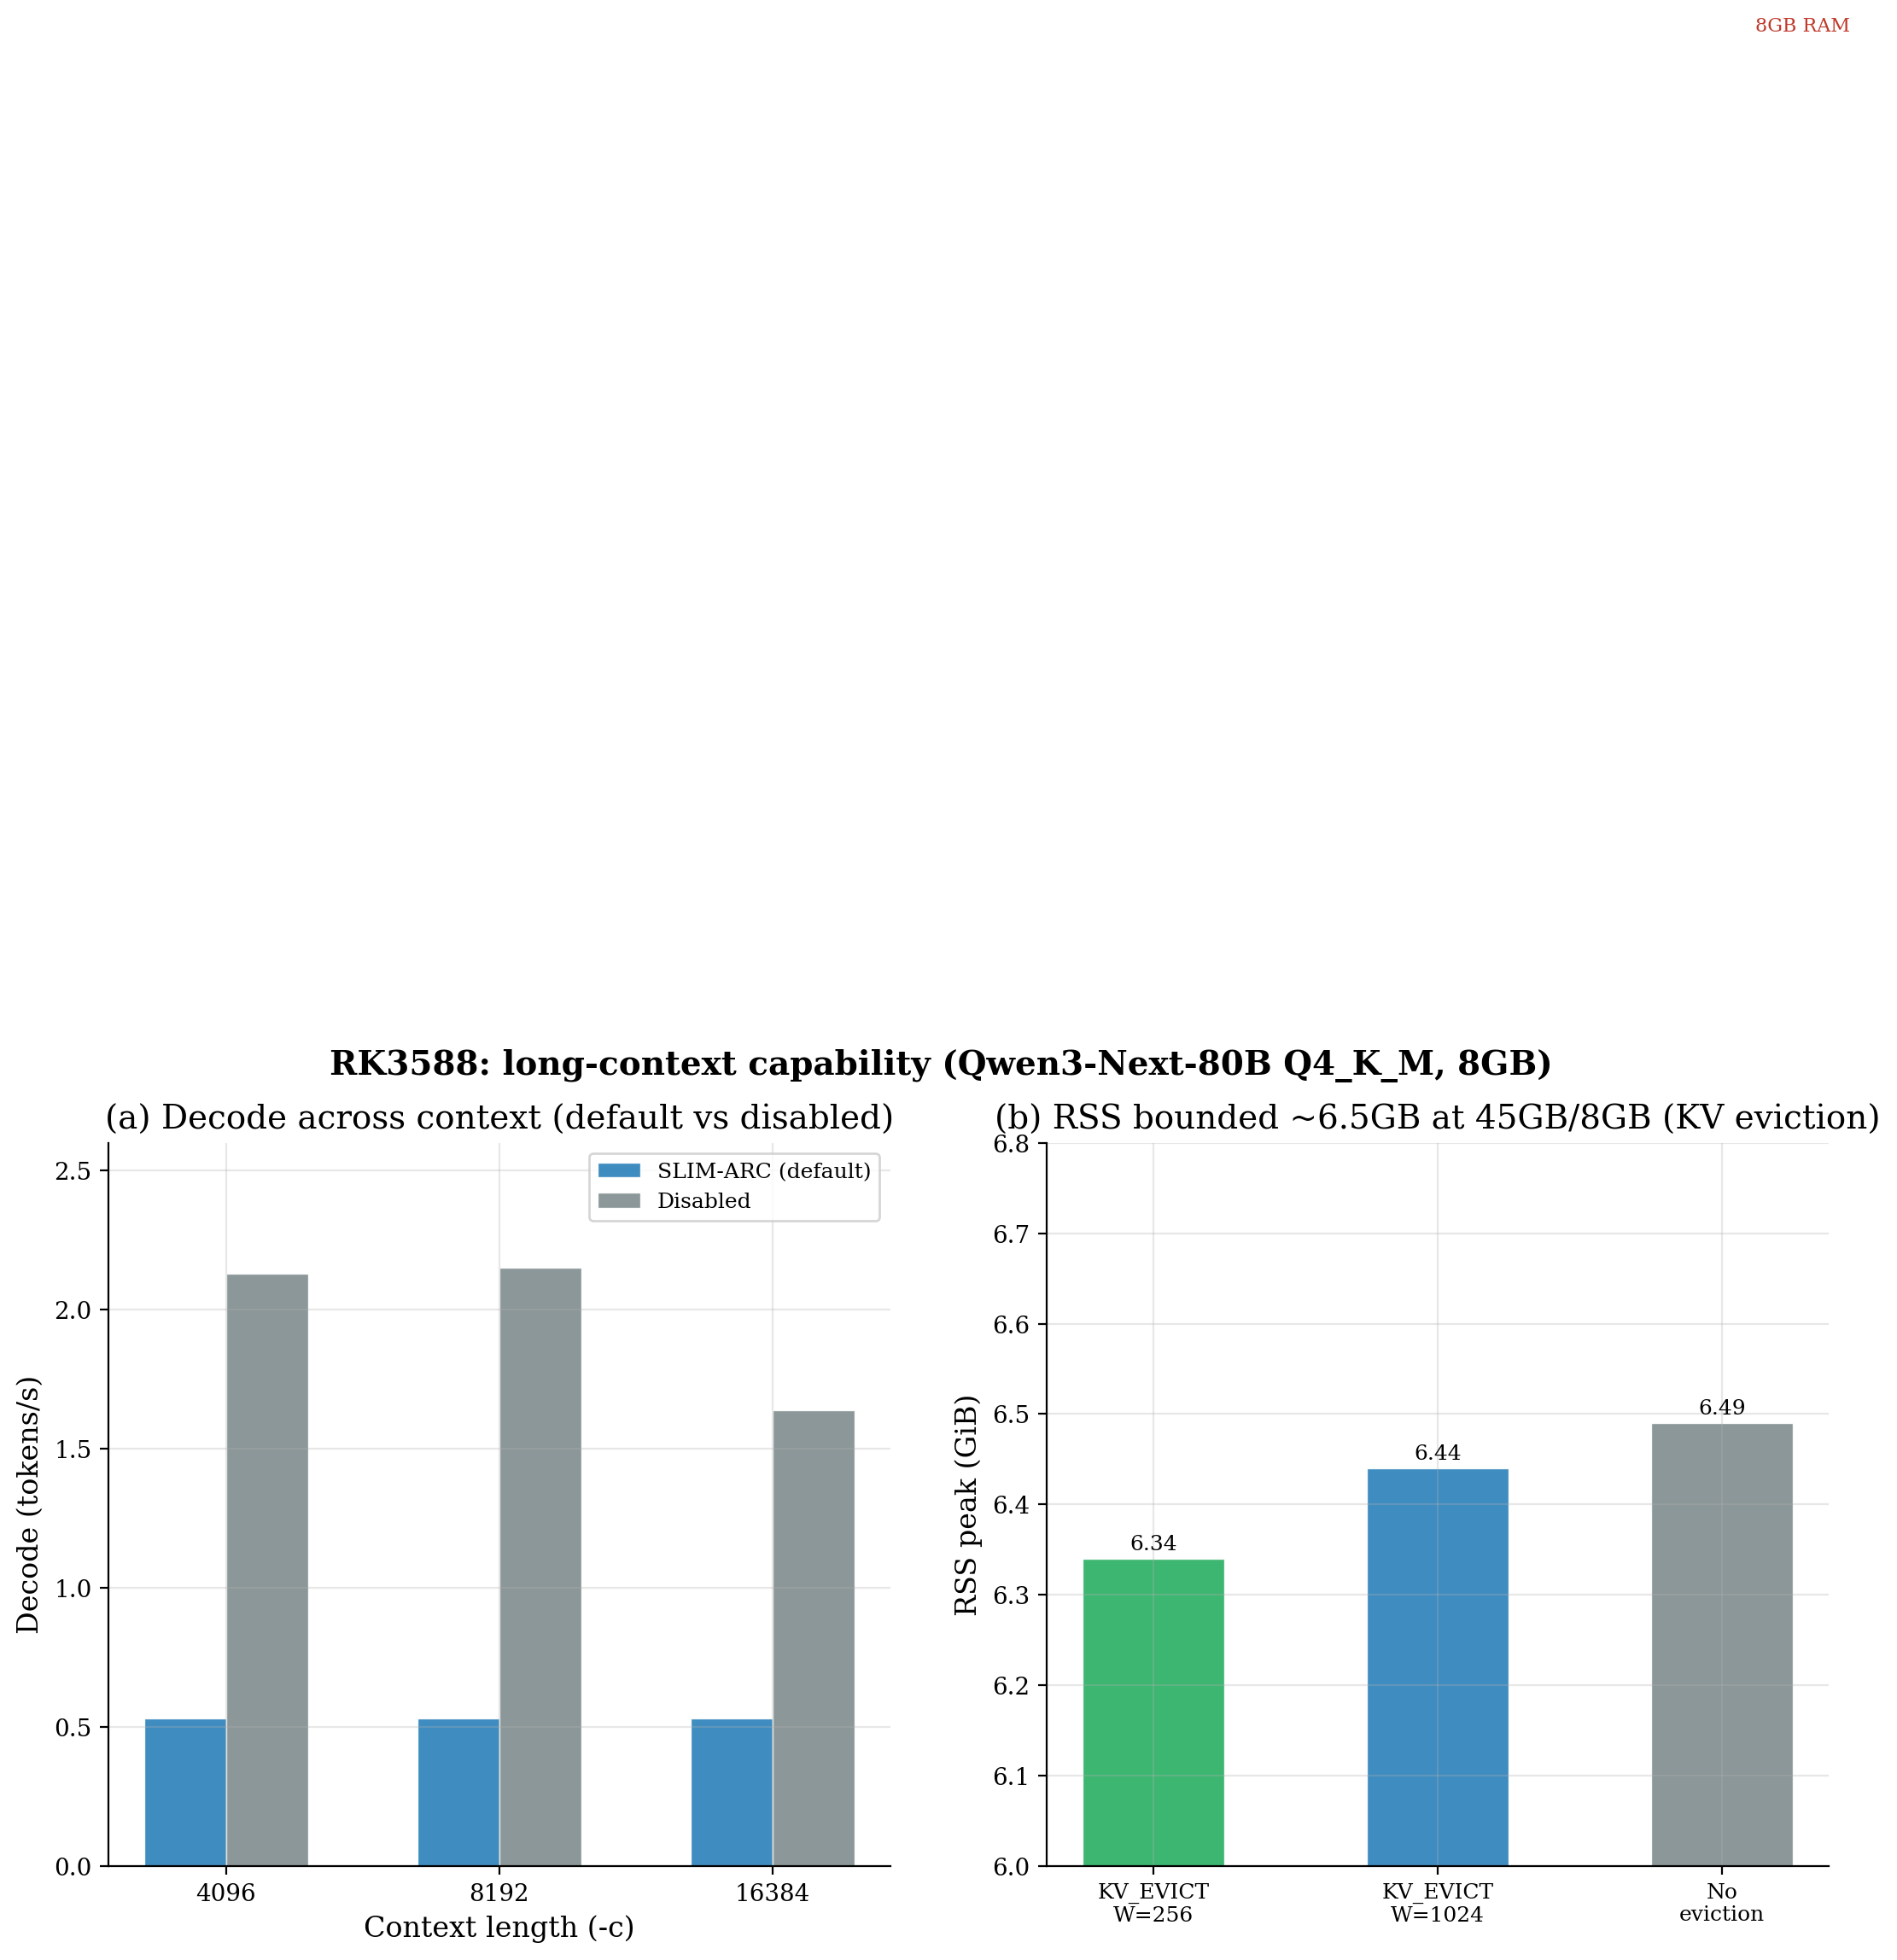
\includegraphics[width=\textwidth]{figures/fig_edge_longctx.png}
    \caption{RK3588 长上下文能力。(a) 45\,GB/8\,GB 极端比例下不同上下文长度的 decode 对比（默认 vs 禁用）；(b) KV eviction 三种配置的 RSS 峰值（6.34--6.49\,GiB，均低于 8\,GB 物理内存，不 OOM）。}
    \label{fig:edge_longctx}
\end{figure}

\subsubsection{专家预取机制排查与改进}

端侧测试还暴露了专家预取机制"触发但无收益"的问题。经排查修复了三个 bug（Router 节点层号解析失败、decode 层范围扫描失败、集成脚本幂等性回归），并通过调试计数确认专家 WILLNEED 实际下发 846 次（修复前为 0）。

\begin{table}[H]
    \centering
    \caption{专家预取改进（n=64 采样，80B Q4\_K\_M）}
    \label{tab:edge_expert}
    \begin{tabular}{lccc}
        \toprule
        \textbf{改进} & \textbf{下发字节} & \textbf{命中率} & \textbf{tg (t/s)} \\
        \midrule
        baseline（temporal 预测） & 27.8\,GB & 31.1\% & 1.9 \\
        \textbf{置信度门控（\texttt{CONF=1}）} & \textbf{12.1\,GB} & \textbf{55.4\%} & 1.9 \\
        统一 I/O 预算（\texttt{BUDGET=1}） & 25.8\,GB & 28.8\% & 1.9 \\
        热门专家并集（\texttt{POP=16}） & 72.6\,GB & 19.3\% & 2.0 \\
        \bottomrule
    \end{tabular}
\end{table}

同时将专家预测器从空间预测（上一层路由 $\to$ 本层，精度 4.5\%）改进为时间预测（同层上一 token 路由 $\to$ 本 token，精度 34.9\%，随机基线约 2\%）。基于文献调查的 4 点改进中，\textbf{置信度门控}（仅预取连续两 token 均激活的稳定专家）使命中率提升 24 个百分点、下发字节减少 56\% 且速度无损，为明确收益；统一 I/O 预算机制正确但端侧非 I/O 受限、收益有限；热门专家并集为诚实负结果（默认关闭）。

\begin{figure}[H]
    \centering
    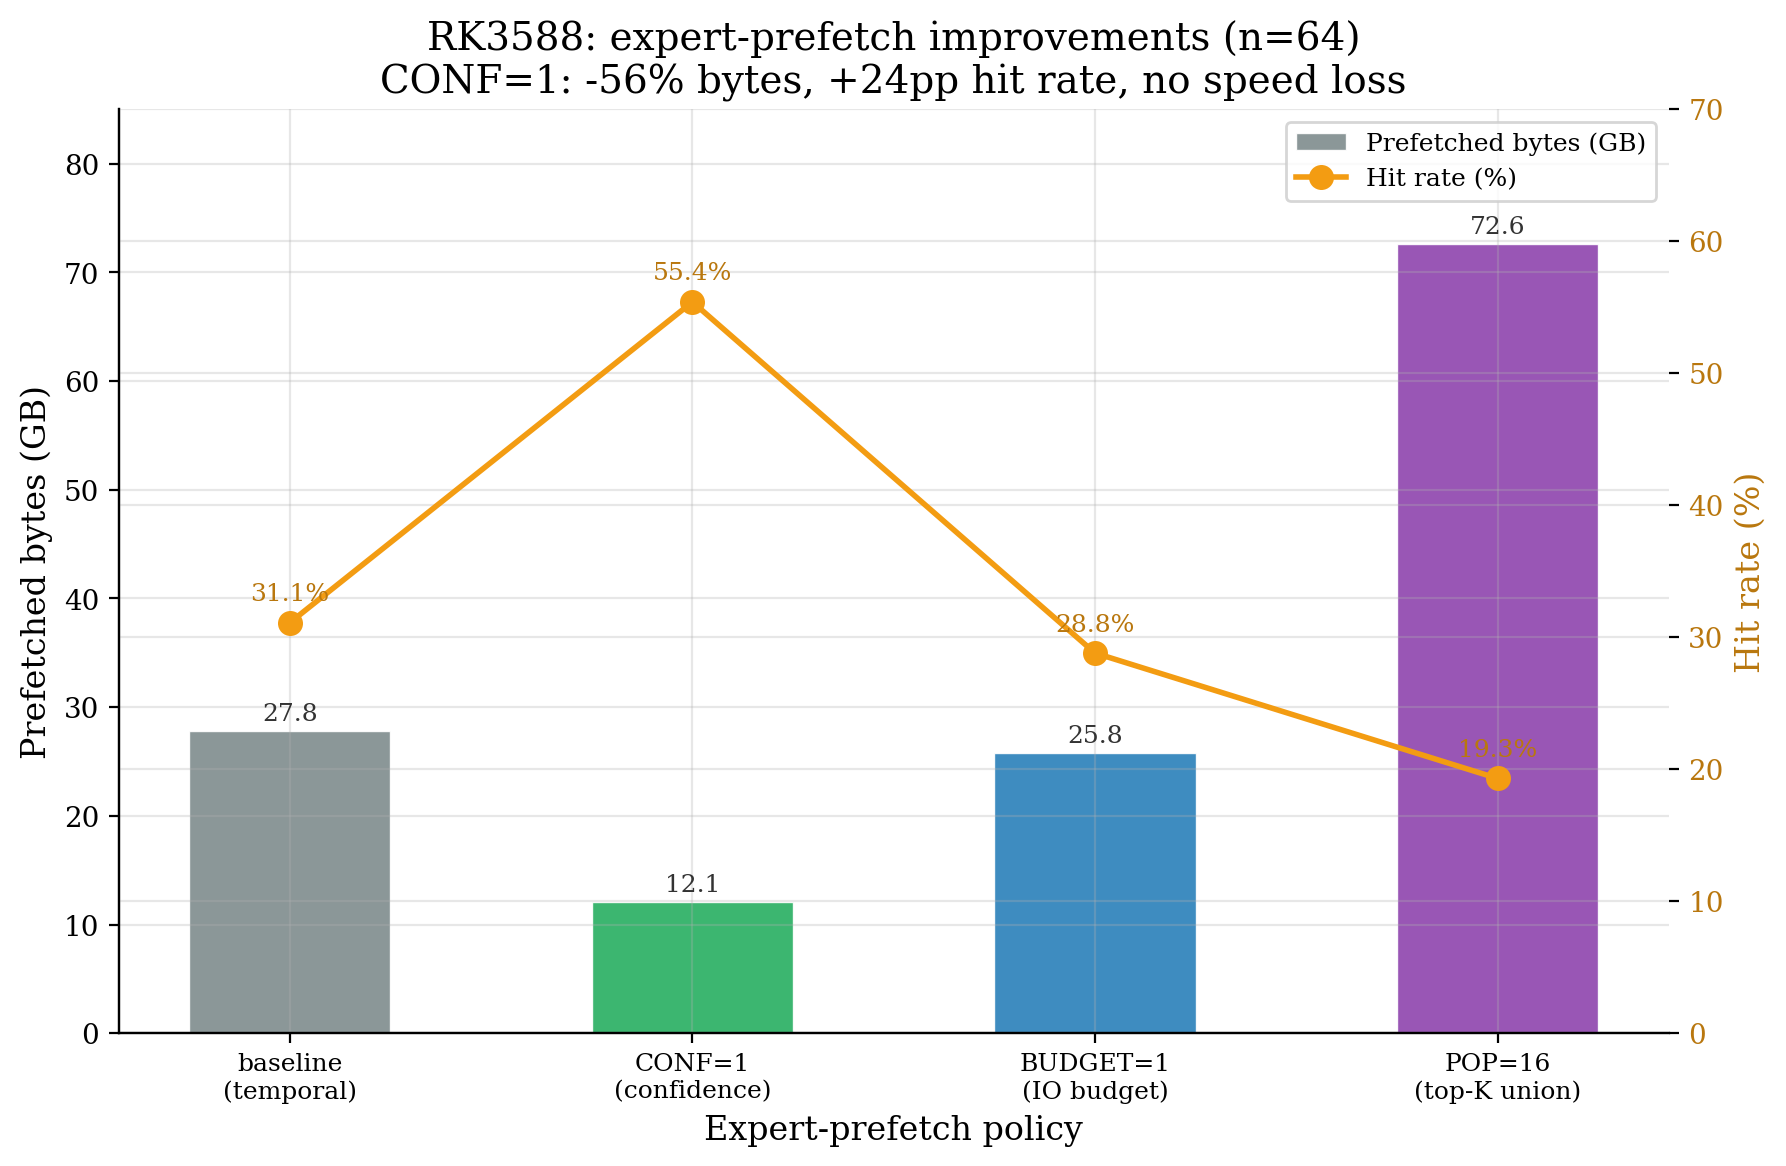
\includegraphics[width=0.9\textwidth]{figures/fig_edge_expert.png}
    \caption{RK3588 专家预取改进对比。置信度门控（CONF=1）将预取字节从 27.8\,GB 降至 12.1\,GB（-56\%）、命中率从 31.1\% 提升至 55.4\%（+24 个百分点）且解码速度无损；统一 I/O 预算（BUDGET=1）机制正确但端侧非 I/O 受限、收益有限；热门专家并集（POP=16）为诚实负结果（默认关闭）。}
    \label{fig:edge_expert}
\end{figure}

\subsubsection{小模型端侧基线}

端侧早期验证（microSD 存储阶段）还测定了小模型基线：Qwen3-4B（2.32\,GB）decode 达 6.90\,t/s，FlashAttention 开启带来约 2$\times$ 提升（tg 3.49$\to$6.90）；OLMoE-1B-7B（4.21\,GB）decode 达 10.7\,t/s，并验证了 MoE 专家预取调用链在端侧安全运行。值得注意的是 KV q4\_0 在 ARM 端侧 decode 反而略慢（6.90$\to$5.05，无 i8mm/SVE），反映量化收益的环境相关性，与 WSL 结论相互印证。

\subsubsection{端侧瓶颈分析与诚实边界}

瓶颈分析（08-08）表明，RK3588 的 80B 解码\textbf{并非 SSD I/O 受限}，而是受计算吞吐/并行度/内存带宽共同限制：线程消融 t4/t6/t8 的解码吞吐为 1.9/1.8/1.3\,t/s（加线程反而变慢）；vmstat 显示解码期 SSD 读约 500--560\,MB/s（容量 2.1\,GB/s 未饱和）、I/O 等待 9--13\%、CPU 空闲 40--45\%。因此 I/O 预取类机制（层预取 + 专家预取 + WILLNEED）对端侧解码提速存在物理上限。

综合来看，SLIM-ARC 在 RK3588 端侧的真实价值为：(1) 消除静态 MADV\_RANDOM 造成的 4--6$\times$ 负优化（动态 MADV 追平禁用）；(2) prefill 提速 10--15\%；(3) 长上下文不 OOM 的能力收益；(4) 专家预取机制经修复后正确触发，置信度门控为明确收益。这与初赛 WSL 环境（MADV\_RANDOM 带来 3.6--5.4$\times$ decode 加速）形成对照，说明 SLIM-ARC 的策略需按"内存比例"而非仅按"是否 MoE"选择——这一发现已沉淀为动态 MADV 与可配置开关，是本项目在真实端侧验证中获得的重要结论。
